\section{Evaluation}\label{sec:evaluation}
%
In this section, we evaluate the performance of adapter synthesis and
present its applications using case studies.
%
In Section~\ref{subsec:case-study-security}, we present an example of finding
adaptable substitutability modulo a bug---enabling programmers to more easily replace buggy
components of their code.
%
In Section~\ref{subsec:rc4-experiment}, we show how our technique can
enable programmers to switch between different libraries with the same
functionality.
%
In Section~\ref{subsec:c-library-evaluation}, we show that adapter
synthesis can find adapters even within a library.
%
In Section~\ref{subsec:conc-search}, we compare symbolic execution-based adapter search
with concrete enumeration-based adapter search.
%
Finally, in Section~\ref{subsec:eval_general}, we show how our technique can be used for
reverse engineering.
\subsection{Case Study: Security}\label{subsec:case-study-security}
%
\lstinputlisting[caption={Two implementations for mapping ordered keys, negative or positive, to values using a C array},
label={lst:lookup}]{chapters/adapter_synthesis/code_samples/lookup.c}
%
%Data structures that map keys to their corresponding values are commonly found in modern programming languages~\cite{hashtbl-ocaml},~\cite{map-cpp}. 
%
%Support for such data structures is not part of the C language standard.
%
%Arrays in C provide a convenient and fast way for mapping a previously known number of integer keys to values.
%
%Implementation of data compression algorithms and signal processing implementations require constant-time lookup for negative and positive powers of values.
%
%In such situations, an array in C can be the perfect solution.
%
Consider a table implementing a function of a signed input.
%
For example, keys ranging from -127 to 127 can be mapped to a 255-element array.
%
Any key \textit{k} will then be mapped to the element at position \textit{k}+127 in this array.
%
We present two implementations of such lookup functions in Listing~\ref{lst:lookup}.
%
Both functions, \textit{lookup1} and \textit{lookup2}, assume keys ranging from $-$\textit{len}/2 to +\textit{len}/2 are mapped in the \textit{table} parameter with \textit{lookup1} being specific to tables of length 255.
%
However, \textit{lookup1} contains a bug caused by undefined behavior.
%
The return value of \textit{abs} for the most negative 32-bit integer~(-2147483648)~is not defined~\cite{gnu-abs}.
%
Given the most negative 32-bit integer, the eglibc-2.19 implementation of \textit{abs} returns that same 32-bit integer.
%
This causes the check on line 2 of Listing~\ref{lst:lookup} to not be satisfied, allowing execution to continue to line 5 and causing an out-of-bounds memory access.
%
\textit{lookup2} in Listing~\ref{lst:lookup} is a different implementation of an array-based lookup with a different interface than \textit{lookup1}.
%
Checking whether the key is in range is done differently in \textit{lookup2}, causing it to not have the memory access bug present in \textit{lookup1}.
%
For this reason, users of \textit{lookup1} may find it desirable to substitute the use of \textit{lookup1} with \textit{lookup2}.
%
Adapter synthesis can perform such a substitution by adapting \textit{lookup2} to \textit{lookup1} while simultaneously not adapting the out-of-bounds memory access in \textit{lookup1}.
%
Our adapter synthesis implementation synthesizes the correct argument substitution adapter in the \textit{lookup1} $\leftarrow$ \textit{lookup2} direction in about 8 minutes.
%
Synthesis of the correct adapter is slowed down by the presence of the \textit{table} pointer in the interfaces of \textit{lookup1} and \textit{lookup2}.
%
The adapter is shown on lines 15-18 of Listing~\ref{lst:lookup}.
%
This case study shows adapter synthesis can replace a buggy function
with its bug-free variant by doing adaptation modulo a bug.
%
\subsection{Case Study: Library Replacement}\label{subsec:rc4-experiment}
%
To show that adapter synthesis can be applied to replace functionality
from one library with that from another library, we adapt functions implementing RC4 functionality in mbedTLS and OpenSSL.
\noindent
\subsubsection{RC4 context initialization} The RC4 algorithm uses a
variable length input key to initialize a table with 256 entries within
the context argument.
%
Both cryptography libraries in our example, mbedTLS and OpenSSL, have their own implementation of this initialization routine.
%
Both initialization function signatures are shown in Figure \ref{fig:rc4setup_adapter}.
%
\begin{figure}[]
	\centering
	\caption{Argument substitution adapter to make \textit{RC4\_set\_key} adaptably equivalent to \textit{mbedtls\_arc4\_setup}}
	\label{fig:rc4setup_adapter}
	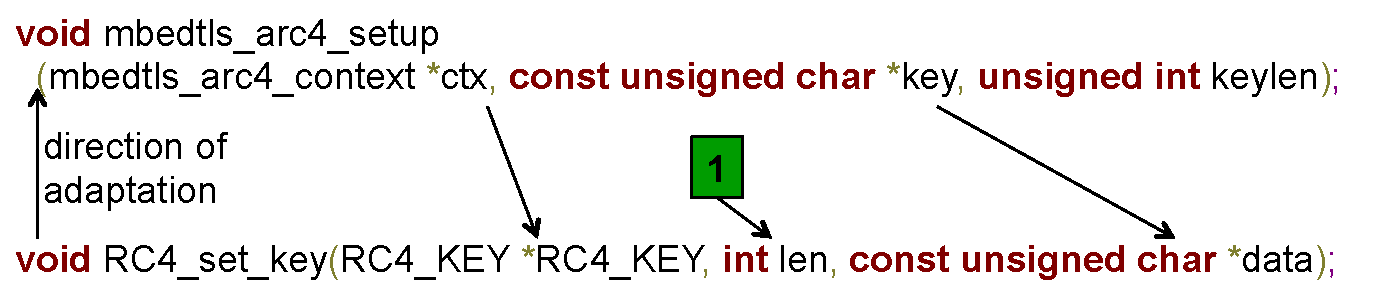
\includegraphics[width=\widthfactor\columnwidth]{chapters/adapter_synthesis/figures/rc4setup_adapter}
\end{figure}
%
Executing each of these initialization routines requires 256 rounds of
mixing bytes from the key string into the context.
%
%Each round requires two load and two store operations into an array with 256 entries.
%
The two initialization routines require the key length and key string arguments at different positions, and use different RC4 context structures (\textit{RC4\_KEY} in OpenSSL, \textit{mbedtls\_arc4\_context} in mbedTLS).
%
The RC4 context arguments contain three fields as shown in Figure \ref{fig:rc4_struct_adapter}.
%
\begin{figure}[]
	\centering
	\caption{Memory substitution adapter to make \textit{RC4\_KEY} adaptably equivalent to \textit{mbedtls\_arc4\_context}}
	\label{fig:rc4_struct_adapter}
	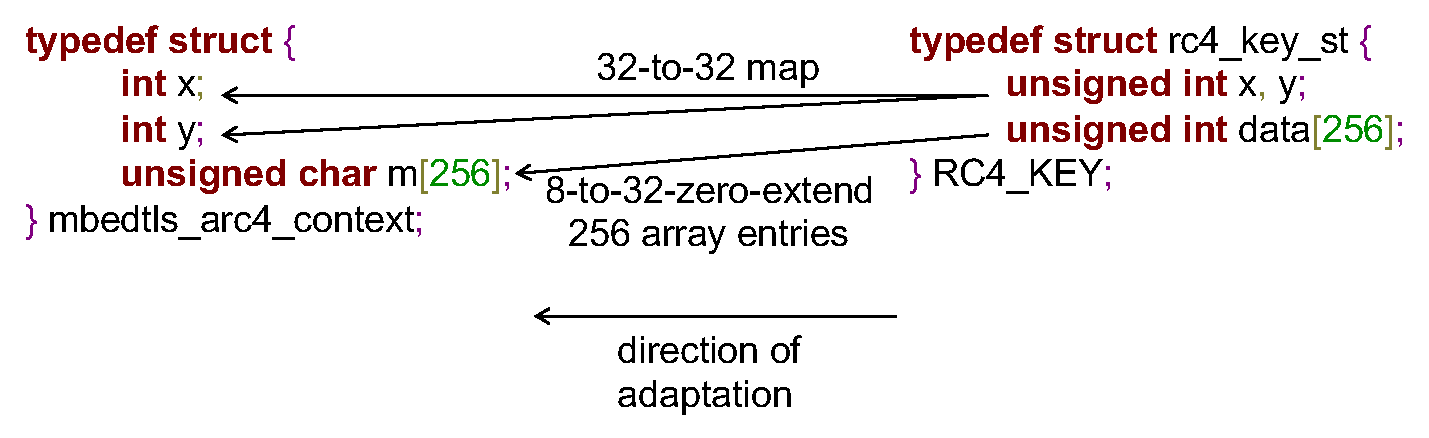
\includegraphics[width=\widthfactor\columnwidth]{chapters/adapter_synthesis/figures/rc4_struct_adapter}
\end{figure}
%
The first two 4-byte fields are used to index into the third field, which is an array with 256 entries.
%
Each entry in the array is 4 bytes wide in OpenSSL and 1 byte wide in mbedTLS.
%
The correct adapter that adapts the OpenSSL context to the mbedTLS
context~(mbedTLS $\leftarrow$ OpenSSL) performs two mapping operations:
(1) it maps the first two mbedTLS context\rq s fields directly to the
first two OpenSSL context\rq s fields and (2) it zero extends each 1 byte
entry in the third field of the mbedTLS context to the corresponding 4
byte entry in the third field of the OpenSSL context.
%
The correct adapter for making the \textit{RC4\_KEY} structure adaptably
equivalent to the \textit{mbedtls\_arc4\_context} structure is shown in Figure \ref{fig:rc4_struct_adapter}.
%
The correct adapter in the reverse direction~(OpenSSL $\leftarrow$ mbedTLS) changes the second mapping operation to map the least significant byte of each 4 byte entry in the third field to the 1 byte entry in its corresponding position.

Performing this adaptation with \textit{mbedtls\_arc4\_setup} and
\textit{RC4\_set\_key}~(the RC4 context initialization functions in
mbedTLS and OpenSSL respectively) requires adaptation of side-effects on memory
because mixing of the key string into the context is the only output of these functions.
%
Since a memory substitution structure can be used both as input and as output, we have to perform the memory substitution adaptation at least twice.
%
First, the reference function may use the memory substitution structure as input.
Hence, we need to adapt the initial byte values of the memory substitution structure to obtain the initial byte values to be used for the reference function.
%
Second, before running the reference function, the target function could have written to the memory substitution structure.
Hence, we need to adapt side-effects of the target function on the memory substitution structure in order to compare them with corresponding side-effects on memory from the reference function.
%
The most general memory substitution adapter synthesis allows arbitrary
numbers of 1, 2, 4, or 8 byte entries in each field of the
264~($2 \times 4 + 256 \times 1$) byte mbedTLS context and 1032~($2 \times 4+256 \times 4$) byte OpenSSL
context.
%
But this makes the search space of memory mappings very large.
%
We instead only explored adapters where the number of entries in each array was a power of 2.
%
While this reduction is useful in practice, it still gives us a search space of about 4.7 million possible memory substitutions in both directions of adaptation.

Finally, memory substitution must be combined with argument substitution to synthesize adapters between \textit{mbedtls\_arc4\_setup} and \textit{RC4\_set\_key}.
%
This combination of argument substitution and memory substitution adapter families creates a search space of 5.593 billion adapters.
%Vaibhav: I got this number of adapters by multiplying 4.7 million memory substitution adapters with the argument substitution number for f1nargs = 3, f2nargs = 3, const_lb = 1, const_ub = 1, return value substitution adapters = 8*f2nargs + 9 + (const_ub - const_lb + 1) + 1. We ran this adapter synthesis with the full return value substitution adapter. The exact calculation code is on mccarran:/export/scratch/vaibhav/tests/calc_num_adaptors.c
%
Our adapter synthesis tool figures out the correct argument,
memory, and return value substitutions.
%
It finds adaptable equivalence in both directions of adaptation by checking equivalence between side-effects on the structure objects~(\textit{ctx} for \textit{mbedtls\_arc4\_setup}, \textit{RC4\_KEY} for \textit{RC4\_set\_key}).
%
The correct adapter for adaptably substituting the
\textit{mbedtls\_arc4\_setup} function with the \textit{RC4\_set\_key}
function is shown in
Figure~\ref{fig:rc4setup_adapter}.
%
To setup adapter synthesis between these two function pairs (we synthesized adapters in both directions), we used a symbolic key string of length 1, and hence the synthesis tool correctly sets the key length argument to 1.
%
While we acknowledge that using an input string of length 1 is too small to be useful, we expect the adapter to be correct on strings of length greater than 1 in practice.
%
We also plan to integrate techniques such as path merging~\cite{KuznetsovKBC2012,AvgerinosRCB2014} to increase the bounds of inputs used in adapter synthesis.
%
While we used an input memory substitution size of 1032 symbolic bytes for memory substitution, both \textit{mbedtls\_arc4\_setup} and \textit{RC4\_set\_key} initialize this memory with concrete values in their implementation, thereby causing this adaptation to start with a much smaller symbolic state consisting of a single symbolic input byte.

We present the time taken to synthesize adapters for RC4 setup function
pairs in Table~\ref{table:rc4-adapter-synthesis-days}.
%
The execution time shown in Table~\ref{table:rc4-adapter-synthesis-days}
for concrete enumeration-based adapter search is the average execution time
taken for adapter synthesis over 10 correctly synthesized adapters for
adapting RC4 setup functions.
%
We performed adapter synthesis using concrete enumeration-based adapter
search 10 times because concrete enumeration-based adapter search
traverses the adapter space in a random order.
%
Using the execution times shown in Table~\ref{table:rc4-adapter-synthesis-days}
and the observation that our adapter synthesis never used more than 1 CPU core
and 4 GB of RAM, we estimated~\cite{amazon-ec2-pricing} the cost of
this computation on a Amazon EC2 instance~(t2-medium).
%
Table~\ref{table:rc4-adapter-synthesis-cost} shows these estimated costs.
%
These costs suggest that automated
adapter search is likely competitive with paying a human programmer to find
and verify the correctness of an adapter at the binary level.
%
The time required for adapter synthesis can be
further reduced by parallelizing the adapter search in concrete
enumeration and reusing the state of adapter search in FuzzBALL-based
adapter search.
%
We discuss this further in Section~\ref{sec:future_work}.
%
%Thus, we combined the memory substitution adapter with the argument substitution adapter family to synthesize adaptable equivalence between the RC4 setup functions.
%
\noindent
%
\begin{table}[]
	\centering
	\caption{Time taken in days for synthesizing adapters between RC4 setup and
	encryption functions in OpenSSL and mbedTLS}
	\label{table:rc4-adapter-synthesis-days}
	\begin{tabular}{|l|l|l|l|l|}
		\hline
		                                                                                        &
	\begin{tabular}[c]{@{}l@{}}setup \\ (M $\leftarrow$ O)\end{tabular} &
	\begin{tabular}[c]{@{}l@{}}setup \\ (O $\leftarrow$ M)\end{tabular} &
	\begin{tabular}[c]{@{}l@{}}enc \\ (M $\leftarrow$ O)\end{tabular} &
	\begin{tabular}[c]{@{}l@{}}enc \\ (O $\leftarrow$ M)\end{tabular} \\
		\hline
		\begin{tabular}[c]{@{}l@{}}Concrete \\ enumeration-based \\ adapter
		search\end{tabular} & 8.24
			& 5.52
			& 5.65
			& 5.52
			\\ \hline
			\begin{tabular}[c]{@{}l@{}}FuzzBALL-based\\  adapter
			search\end{tabular}                & 7.87
				& 6.15
				& 8.54
				& 2.10
				\\ \hline
			\end{tabular}
		\end{table}

\begin{table}[]
	\centering
\caption{Estimated cost~(in USD) of synthesizing adapters between RC4 setup and encryption functions in OpenSSL and mbedTLS on an Amazon EC2 instance}
\label{table:rc4-adapter-synthesis-cost}
			\begin{tabular}{|l|c|c|c|c|c|}
				\hline
				                                                                                    &
				\begin{tabular}[c]{@{}c@{}}setup \\ M $\leftarrow$
				O\end{tabular} & \begin{tabular}[c]{@{}c@{}}setup \\ O
				$\leftarrow$ M\end{tabular} & \begin{tabular}[c]{@{}c@{}}enc \\
				M $\leftarrow$ O\end{tabular} & \begin{tabular}[c]{@{}c@{}}enc
				\\ O $\leftarrow$ M\end{tabular} & Total   \\ \hline
					\begin{tabular}[c]{@{}l@{}}Concrete \\ enum.-based \\
					adapter\\ search\end{tabular} & \$9.17
						& \$6.15
						& \$6.29
						& \$6.15
						& \$27.76 \\ \hline
						\begin{tabular}[c]{@{}l@{}}FuzzBALL-\\ based\\ adapter\\
						search\end{tabular}        & \$8.76
							& \$6.84
							& \$9.51
							& \$2.34
							& \$27.45 \\ \hline
						\end{tabular}
					\end{table}

%
\subsubsection{RC4 encryption} The RC4 encryption functions in mbedTLS and
OpenSSL take 4 arguments each, three of which are pointers to the RC4
context, the input key string, and the output string, as shown in
Figure~\ref{fig:rc4-encrypt-mo}.
%
\begin{figure}[]
	\centering
	\caption{Adapter performing argument and memory substitution to make
	\textit{mbedtls\_crypt} in the mbedTLS library adaptably substitutable
	by \textit{RC4} in OpenSSL}
	\label{fig:rc4-encrypt-mo}
	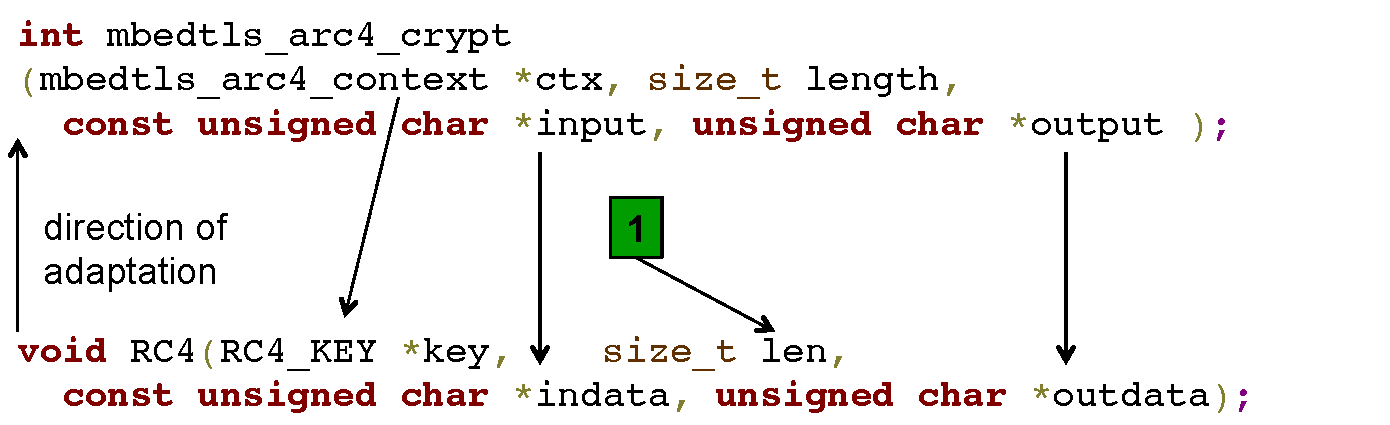
\includegraphics[width=\widthfactor\columnwidth]{chapters/adapter_synthesis/figures/rc4-encrypt-mo}
\end{figure}
%
These functions use the RC4 context as input, causing the initial symbolic state to consist of 1032 symbolic bytes for memory substitution and one symbolic byte for the input string.
%
These functions both read from and write to the RC4 context, making
two memory substitution adaptations necessary.
%
These functions also encrypt every byte of the input string using a loop where the length of the input string is given as a parameter to the function.
%
Since all arguments to the reference function are symbolic, using a symbolic formula for the length of the input string can easily cause the loop bound to be very large, especially if the symbolic formula for the length allows the possibility of the length being equal to one of the pointer arguments to the reference function.
%
To avoid the encryption loop in the reference function from executing too many times, we restricted every instruction in the reference function to be executed at most twice.
%
Finally, because these functions write to an output string, it is
necessary for us to have memory side-effects equivalence checking to
capture outputs that are not part of the return value.

The adapter search space in this case consists of $1.792 \times 10^{12}$ adapters.
%Vaibhav: I got this number by by multiplying 4.7 million memory substitution adapters with the argument substitution number for f1nargs = 4, f2nargs = 4, const_lb = 0, const_ub = 5, return value substitution adapters = 8*f2nargs + 9 + (const_ub - const_lb + 1) + 1. We ran this adapter synthesis with the full return value substitution adapter. The exact calculation code is on mccarran:/export/scratch/vaibhav/tests/calc_num_adaptors.c 
%
The correct adapter for making the \textit{RC4} method adaptably
equivalent to \textit{mbedtls\_arc4\_crypt} is shown in Figure
\ref{fig:rc4-encrypt-mo}.
%
Our adapter synthesis tool finds the correct argument and memory
substitution adapters in both directions of adaptation.
%
Tables~\ref{table:rc4-adapter-synthesis-days},~\ref{table:rc4-adapter-synthesis-cost}
show the time taken for and estimated cost of adapter synthesis between
the RC4 encryption functions in OpenSSL and mbedTLS.
%
Once again, the execution time shown in Table~\ref{table:rc4-adapter-synthesis-days}
for concrete enumeration-based adapter search is the average execution time
taken for adapter synthesis over 10 correctly synthesized adapters.
%
We verified the correctness of our adapted context structures by using self-tests present in mbedTLS and OpenSSL.
%
%Given the design of the RC4 encryption algorithm, we do not expect the correctness of our adapters to change for longer input strings.
%
\noindent
\subsubsection{On improving memory substitution performance} On
combining the memory substitution adapter family with argument and
return value substitution, our adapter synthesis tool encountered a
significant slowdown with both RC4 context initialization and encryption.
%
This can be attributed in part to the encoding of memory substitutions in our tool.
%
We enumerate all possibilities of memory substitutions into the formula of every byte in the memory substitution structure, causing the symbolic formulas to be very large.
%
We plan to encode the memory substitution adapter more efficiently in the future to make better use of existing solvers.
%
Another significant cause of the slowdown, in the case of RC4 context initialization, is the slow symbolic execution of 256 rounds of key mixing, once in the target and once in the reference function, because of two symbolic loads and two symbolic stores to memory on every round of key mixing.
%
We plan to integrate loop summarization~(for example, as described by
Godefroid et al.~\cite{godefroid2011}), and use the theory of arrays for symbolically-indexed memory accesses to speed up this symbolic execution in the future.
%
In the case of RC4 encryption, since we have to adapt the memory substitution structures twice (once for input and once for output) we have to present large formulas to the solver at least twice on every execution path with each query taking a few seconds.
%
This large symbolic state is the cause of significant slowdown during RC4 encryption adapter synthesis.
%
We plan to explore concretization heuristics of symbolic bytes in the future to reduce the number of solver invocations made during RC4 encryption adapter synthesis.
%
\noindent
\subsubsection{RC4 adapter verification using nmap} We verified the
correctness of our RC4 memory substitution adapter using nmap with the setup shown in Figure \ref{fig:nmap_struct_adapter}.
%
\begin{figure}[]
	\centering
	\caption{nmap using RC4 encryption in mbedTLS instead of OpenSSL}
	\label{fig:nmap_struct_adapter}
	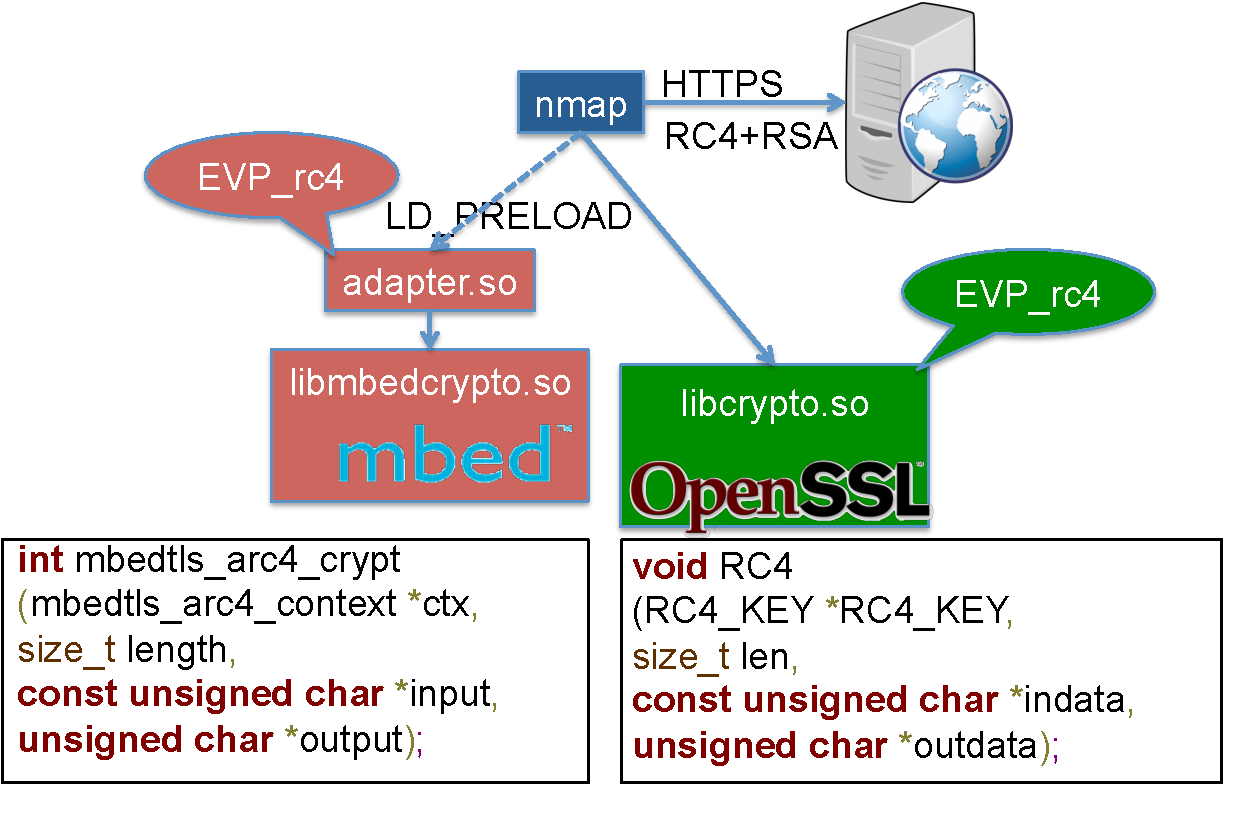
\includegraphics[width=\widthfactor\columnwidth]{chapters/adapter_synthesis/figures/nmap_struct_adapter}
\end{figure}
%
We created adapted versions of the OpenSSL RC4 setup and encryption
functions that internally use the mbedTLS context adapted to the OpenSSL
context.
%
On a 64-bit virtual machine running Ubuntu 14.04, we compiled the adapted setup and encryption functions into a shared library and setup a local webserver, which communicated over port 443 using the \textit{RC4+RSA} cipher.
%
We used the stock nmap binary to scan our localhost and injected our specially created shared library using the \textit{LD\_PRELOAD} environment variable.
%
The preloading caused the RC4 functions in our shared library to be executed instead of the ones inside OpenSSL.
%
The output of nmap, run with preloading our specially created shared library which used the OpenSSL $\leftarrow$ mbedTLS structure adapter, was the same as the output of nmap when using the system OpenSSL library.
%
\subsection{Intra-library Adapter Synthesis}
\label{subsec:c-library-evaluation}
%
The previous section showed an application of adapter synthesis where the target and reference functions came from
independently-developed implementations.
%
But, adapter synthesis can also be useful in cases where the target and reference functions were developed within the same
library.
%
Synthesizing adapters between binary functions in the same library can expose important relations between adaptably
substitutable functions that may not be known to users of the library.
%
It can show relations between functions, by, for example showing that one function can be adaptably
implemented in terms of another.
%
Verifying such relations between functions from their binary implementation can provide the users of the library a
more detailed picture of the function\rq s behavior.
%
In libraries with a large interface, such as the Ubuntu 14.04 system C library, where it can be challenging to manually identify
adaptability relations between functions, performing automated intra-library adapter synthesis can be particularly
useful.
%
\subsubsection{Setup}
%
We evaluated our adapter synthesis tool on the system C library available on Ubuntu 14.04~(eglibc 2.19).
%
The C library uses a significant amount of inlined assembly, for instance, the \textit{ffs}, \textit{ffsl}, \textit{ffsll} functions, which
motivates automated adapter synthesis at the binary level.
%
We enumerated 1316 exported functions in the library in the order they
appear, which caused functions that are defined in the same source files
to appear close to each other.
%
Considering every function in this list as the target function, we chose five functions that appear above and below it as 10 potential reference functions.
%
These steps gave us a list of 13130~($10\times 1316 - 2 \times \sum_{i=1}^5 i$) pairs of target and reference functions.
%since the first five and the last five target functions 
%had less than five potential semantically-equivalent reference functions. 
%
We used the argument substitution and type conversion adapter families combined with the return value adapter family because these families scale well and are widely applicable.
%
We ran our adapter synthesis with a 2 minute timeout on a machine running CentOS 6.8 with 64-bit Linux kernel version 2.6.32 using 64 GB RAM and a Intel Xeon E5-2680v3 processor.
%
To keep the running time of the entire adapter synthesis process within practical limits, we configured FuzzBALL to use a 5 second SMT solver timeout and to consider any queries that trigger this timeout as unsatisfiable.
%
We limited the maximum number of times any instruction can be executed to 4000 because this allowed execution of code which loaded library dependencies.
%
We limited memory regions to be symbolic up to a 936 byte offset limit (the size of the largest structure in the library interface) and any offset outside this range was considered to contain zero.
%
\subsubsection{Results}
%
Table~\ref{table:libc-evaluation} summarizes the results of searching for argument substitution and type conversion adapters with a return value adapter within the 13130 function pairs described above.
%
The similarity in the results for the type conversion adapter family and argument substitution adapter family arises from the similarity of these two families.
%
%We synthesized the argument substitition adapter, with and without type conversion, along with the return value adapter.
%However, trying to synthesize an adapter using a simpler grammar translates into simpler queries for the solver, which in turn, results in the adapter synthesis tool concluding with a result of equivalence or the lack of it within the two minute hard timeout.
%
%For about 69\% of the 13130 function pairs, our synthesis tool concluded that functional equivalence cannot be created between the target and reference functions for the chosen adapter grammar.
%
%Our adapter synthesis tool timed out for about 21\% of the function pairs.
%
The most common causes of crashing during execution of the target function were missing system call support in FuzzBALL and incorrect null dereferences~(caused due to lack of proper initialization of pointer arguments).
%
The timeout column includes all function pairs for which we had a solver timeout~(5 seconds), hit the iteration limit~(4000), or reached a hard timeout~(2 minutes).
%
The search terminated without a timeout for 70\% of the function pairs, which reflects a complete exploration of the space of symbolic inputs to a function, or of adapters.
%Because our test harness executes the target function first, in some cases, FuzzBALL failed to execute any execution paths to completion before starting execution of the reference function.
%
%While missing system call functionality in FuzzBALL was one cause for these failures, FuzzBALL often incorrectly classified pointer argument dereferences in the target function as null dereferences which caused the execution path to terminate.
%
%Another cause of failure to execute any execution paths through the target function to completion was the iteration limit of 4000 we used during our experiments.
%
%Our adapter synthesis tool reports 391 and 392 adapters for the argument substition grammar without type conversion and with type conversion respectively.
%
%
%
%We present the true positives found by our C library evaluation in the next subsection.
%
%But, during the last counter-example search step for the reported adapter, not every execution path completed execution through the target function.
%
%If a counter-example search for an adapter finishes executing the target function during every execution path and still fails to find a counter-example, it guarantees that no 
%
%Therefore, we report the number of adapters - 175 out of 391 in case of simple and 174 out of 392 in case of type conversion adapters - for which every execution path during the the final counter-example search step completed execution through the target function.

% One of the the most interesting conclusions from our adapter synthesis tool
% was the adapters reported between the 13130 function pairs, of which
% 2.8\% and 2.7\% were reported to have an adapter when using the argument
% substitution grammar without type conversion and with type conversion respectively.
%
\begin{table}[t]
	\centering
	\caption{Adapter Synthesis over 13130 function pairs without memory-based equivalence checking}
	\label{table:libc-evaluation}
	\begin{tabular}{|l|l|l|l|l|l|}
		\hline
		\begin{tabular}[c]{@{}l@{}}adapter \\ type\end{tabular}     &
		Inequiv. & \begin{tabular}[c]{@{}l@{}}adapters\\ Found\end{tabular}
		& Timeout & \begin{tabular}[c]{@{}l@{}}Target \\ function\\
		crashed\end{tabular} \\ \hline
		\begin{tabular}[c]{@{}l@{}} arg. sub.\end{tabular} & 8887
		& 382 & 3014 &
		847 \\
		\hline
		type conv.  & 8909
		& 383 & 2989 &
		849 \\
		\hline
	\end{tabular}
\end{table}
%
Since there is no ground truth, we manually corroborated the results of our evaluation by checking the C library documentation and source code.
%
Our adapter synthesis evaluation on the C library reported 30 interesting true positives shown in Table~\ref{table:libc-adapters}.
The remaining adapters found were correct, but trivial.
The first column in Table~\ref{table:libc-adapters} shows the function pair between which an adapter was
found (with the number of arguments) and the second
column shows the adapter.
We use the following notation to describe adapters in a compact way.
%
$f_1$ $\leftrightarrow$ $f_2$ means $f_1$ $\leftarrow$ $f_2$ and $f_2$ $\leftarrow$ $f_1$.
%
\# followed by a number indicates reference argument substitution by a target argument, while other numbers indicate constants.
%
X-to-YS represents taking the low X bits and sign extending them to Y bits, X-to-YZ represents a similar operation using zero extension.


%the numbers in the above table's Timeout column include iteration limit timeouts 
%these were derived using the check_iterlimit.cpp file at MSI

%we reduce the number of inequivalences by 34 because that is the number of function pairs
% for which the words "after too many" was found in the log of that function pair
% but near the end of that function pair's log, we found them to be inequivalent

%similar logic was applied in check_iterlimit.cpp for function pairs with "missing results from check run" and for function pairs for which a "Final adapter" was reported

%finally, adding the search string "Solver died with result code 134" instead of "after too many" allowed us to search for number of solver timeouts

%the final numbers in the table are harvest_results[ineq|missing|final] - `grep "ineq: |missing results: | final: " results/<simple-1 or typeconv-4>/iterlimit_solvertimeout.txt` for the 3 columns, ineq, missing results, final adapter. The total of these 3 subtractions was added to the Timeout column. 

\begin{table*}[!htbp]
    \centering
\caption{adapters found within eglibc-2.19}
\label{table:libc-adapters}
%\resizebox{0.6\columnwidth}{!}{%
\begin{tabular}{ll}
\hline
$f_1$ $\leftarrow$ $f_2$ or $f_1$ $\leftrightarrow$ $f_2$                                                                                                                                                                      & adapter                                                                                   \\ \hline
\begin{tabular}[c]{@{}l@{}}abs(1) $\leftarrow$ labs(1)\\ abs(1) $\leftarrow$ llabs(1)\end{tabular}                                                                                                                             & \begin{tabular}[c]{@{}l@{}}32-to-64S(\#0) and \\ 32-to-64Z(return value)\end{tabular}     \\ \hline
\begin{tabular}[c]{@{}l@{}}labs(1) $\leftrightarrow$ llabs(1)\end{tabular}                                                                                                                           & \#0                                                                                       \\ \hline
\begin{tabular}[c]{@{}l@{}}ldiv(1) $\leftrightarrow$ lldiv(1)\end{tabular}                                                                                                                           & \#0                                                                                       \\ \hline
\begin{tabular}[c]{@{}l@{}}ffs(1) $\leftarrow$ ffsl(1)\\ ffs(1) $\leftarrow$ ffsll(1)\end{tabular}                                                                                                                              & 32-to-64S(\#0)                                                                            \\ \hline
\begin{tabular}[c]{@{}l@{}}ffsl(1) $\leftrightarrow$ ffsll(1)\end{tabular}                                                                                                                           & \#0                                                                                       \\ \hline
setpgrp(0) $\leftarrow$ setpgid(2)                                                                                                                                                                            & 0, 0                                                                                    \\ \hline
wait(1) $\leftarrow$ waitpid(3)                                                                                                                                                                               & -1, \#0, 0                                                                               \\ \hline
wait(1) $\leftarrow$ wait4(4)                                                                                                                                                                                 & -1, \#0, 0, 0                                                                          \\ \hline
waitpid(3) $\leftarrow$ wait4(4)                                                                                                                                                                              & \#0, \#1, \#2, 0                                                                        \\ \hline
wait(1) $\leftarrow$ wait3(3)                                                                                                                                                                                 & \#0, 0, 0                                                                               \\ \hline
wait3(3) $\leftarrow$ wait4(4)                                                                                                                                                                                & -1, \#0, \#1, \#2                                                                       \\ \hline
umount(1) $\leftarrow$ umount2(2)                                                                                                                                                                             & \#0, 0                                                                                  \\ \hline
\begin{tabular}[c]{@{}l@{}}putchar(1) $\leftrightarrow$ putchar\_unlocked\\ putwchar(1) $\leftrightarrow$ putwchar\_unlocked(1) \end{tabular} & \#0                                                                                       \\ \hline
\begin{tabular}[c]{@{}l@{}}recv(4) $\leftarrow$ recvfrom(6)\\ send(4) $\leftarrow$ sendto(6)\end{tabular}                                                                                                            & \begin{tabular}[c]{@{}l@{}}32-to-64S(\#0), \#1, \#2, \\ 32-to-64S(\#3), 0, 0\end{tabular} \\ \hline
\begin{tabular}[c]{@{}l@{}}atol(1) $\leftrightarrow$ atoll(1)\end{tabular}                                                                                                            & \begin{tabular}[c]{@{}l@{}}\#0\end{tabular} \\ \hline
\begin{tabular}[c]{@{}l@{}}atol(1) $\leftarrow$ strtol(3)\\ atoi(1) $\leftarrow$ strtol(3) \\ atoll(1) $\leftarrow$ strtoll(3) \end{tabular}                                                           & \begin{tabular}[c]{@{}l@{}}\#0, 0, 10 \end{tabular} \\ \hline \hline
isupper(1) $\leftarrow$ islower(1)                                                                                                                                                                            & \#0 + 32                                                                                  \\ \hline
islower(1) $\leftarrow$ isupper(1)                                                                                                                                                                            & \#0 - 32                                                                                  \\ \hline
killpg(1) $\leftarrow$ kill(1)                                                                                                                                                                            & -\#0, \#1                                                                                  \\ \hline
\end{tabular}
%}
\end{table*}


The last three rows shown in Table \ref{table:libc-adapters} shows three arithmetic adapters found within the C library using partial automation.
%
The functions \textit{isupper}, \textit{islower}, \textit{kill} have assumptions about conditions that will be satisifed by inputs given to them.
% 
We synthesized the correct adapters by writing wrappers containing preconditions around these three functions. %\textit{isupper}, \textit{islower}, \textit{kill} functions.
%
\subsection{Comparison with Concrete Enumeration-based Adapter Search}
\label{subsec:conc-search}
For every adapter family that we have discussed, the space of possible adapters is finite.
%
So instead of using symbolic execution for adapter search, we can find candidate adapters by enumerating concrete adapters until we find one that produces equal side-effects and return values for all previously-found tests.
%
We implement concrete enumeration-based adapter search in C for all the adapter families described in Section~\ref{sec:adapter_synthesis}.
%
We use the Pin~\cite{pin} framework for checking side-effects on memory and system calls for equality.
%
To prevent adapter search time from depending on the order of enumeration, we randomize the sequence in which adapters are generated, ensuring that every adapter had the same probability of being generated.
%
For the adaptable function pairs reported in Section~\ref{subsec:c-library-evaluation}, we synthesized adapters from the type conversion adapter family using both the concrete enumeration- and symbolic execution-based adapter search implementations and captured the total adapter search time.
%
We also counted the size of the adapter search space for every adaptation.
%
In some cases, the adapter search space was too large to be concretely enumerated.
%
For example, the adapter search space for the \textit{killpg} $\leftarrow$ \textit{kill} adapter consists of 98.1 million arithmetic adapters.
%
In such cases, we reduced the size of the search space by using smaller constant bounds.
%
Based on the size of adapter search space, we compared the total adapter search times for both adapter search strategies.
%
We present the results from this comparison in Figure~\ref{fig:conc_vs_se}.
%
\begin{figure}[t]
	\centering
	\caption{Comparing concrete enumeration-based adapter search with binary
	symbolic execution-based adapter search for adapters presented in
	Section~\ref{subsec:c-library-evaluation}}
	\label{fig:conc_vs_se}
	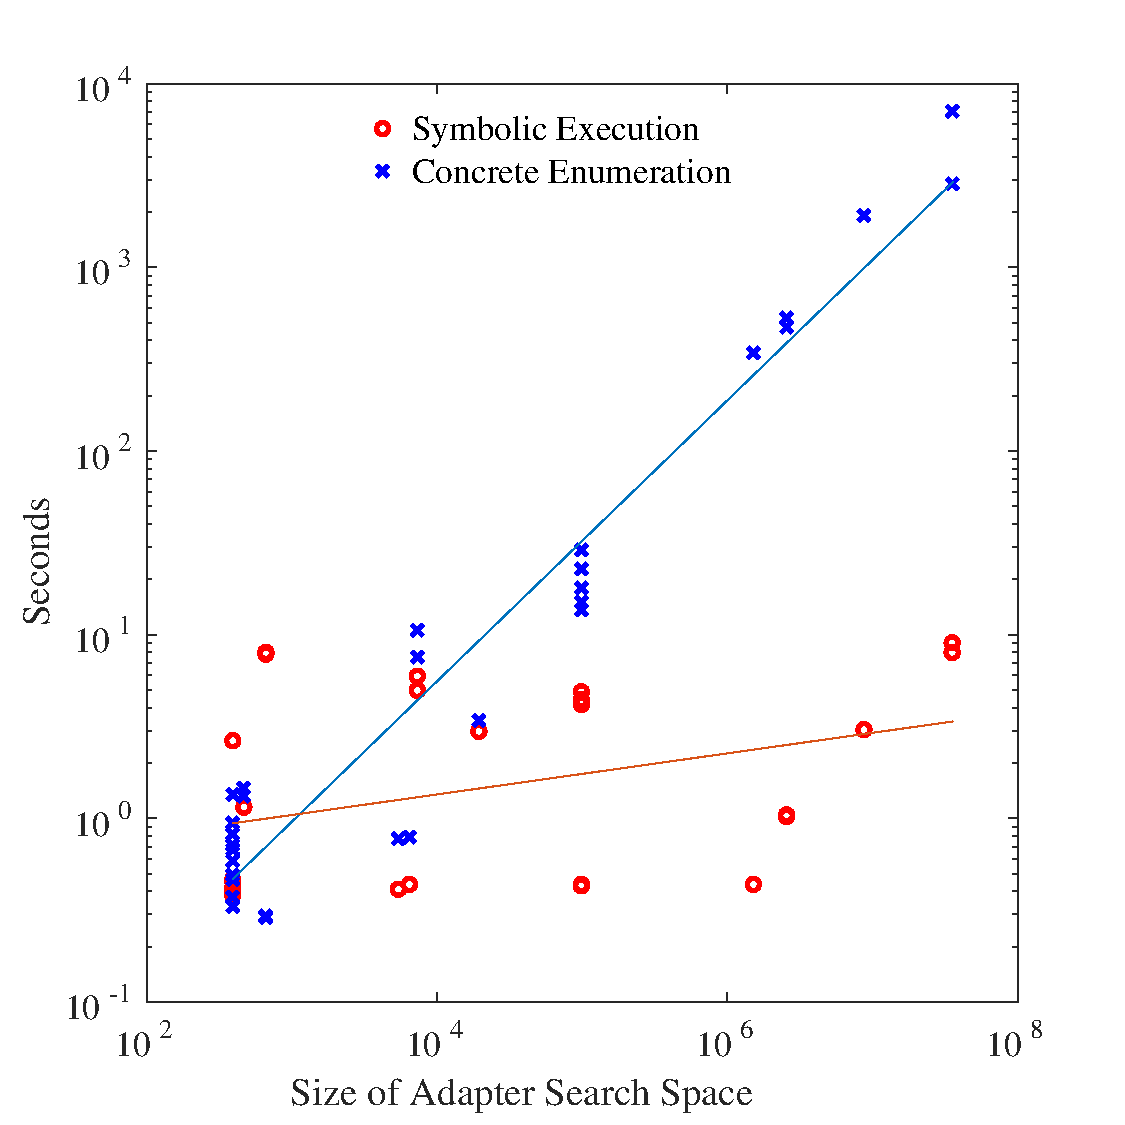
\includegraphics[width=\widthfactor\columnwidth]{chapters/adapter_synthesis/figures/conc_vs_se}
\end{figure}
%
For concrete enumeration-based adapter search, Figure~\ref{fig:conc_vs_se} shows the time required to find an adapter has a consistent exponential increase with an increase in the size of adapter search space.
%
But when using binary symbolic execution-based adapter search,
Figure~\ref{fig:conc_vs_se} shows a much slower increase in time
required to find the adapter.
%
This occurs because symbolic execution is less
affected by an increase in the size of the adapter search space
due to an increase in the number of arguments and the number of
possible constants in the adapter family.
%
\subsection{Large-Scale Reverse Engineering}
\label{subsec:eval_general}
In this section, we show how adapter synthesis can be used for reverse engineering.
Our goal is to understand the behavior of fragments of binary code by synthesizing adapters between those fragments and reference functions with known behavior.
We evaluate on binary code fragments taken from a ARM firmware image and reference functions
chosen from the source code of a popular media player.
\subsubsection{Code fragment selection}
Rockbox~\cite{rockbox} is a free replacement 3rd party firmware for digital music players.
%
We used a Rockbox image compiled for the iPod Nano (2g) device, based on the 32-bit ARM architecture, and disassembled it.
%
We dissected the firmware image into code fragments using the following rules:
%
(1) no code fragment could use memory, stack, floating-point, coprocessor, or supervisor call instructions,
%
(2) no code fragment could branch to an address outside itself,
%
(3) the first instruction of a code fragment could not be conditionally executed.

The first rule disallowed code fragments from having any inputs from/outputs to memory, thereby allowing us to use the 13 general purpose registers on ARM as inputs.
%
The second rule prevented a branch to an invalid address.
%
ARM instructions can be executed based on a condition code specified in the instruction. If the condition is not satisfied, the instruction is turned into a {\tt noop}.
%
The third rule disallowed the possibility of having code fragments that begin with a {\tt noop} instruction, or whose behavior depends on a condition.
%
The outputs of every code fragment were the last (up to) three registers written to by the code fragment.
%
This caused each code fragment to be used as the target code region up to three times, once for each output register.
%
This procedure gave us a total of 183,653 code regions, with 61,680 of them consisting of between 3 and 20 ARM instructions.

To evaluate which code fragments could be synthesized just with our
adapter family without a contribution from a reference function, we
checked
which of these 61,680 code fragments could be adaptably substituted by a reference function that simply returns one of its arguments.
%
Intuitively, any code fragment that can be adaptably substituted by an
uninteresting reference function must be uninteresting itself, and so
need not be considered further.
%
We found 46,831 of the 61,680 code fragments could not be adaptably
substituted by our simple reference function, and so we focused our
further evaluation on these 46,831 code fragments that were between 3
and 20 ARM instructions long and non-trivial.\\
%
\subsubsection{Reference functions}
Since our code fragments consisted of between 3 and 20 ARM instructions, we focused on using reference functions that can be expressed in a similar number of ARM instructions.
%
We used the source code of version 2.2.6 of the VLC media player~\cite{vlc} as the codebase for our reference functions.
%
We performed an automated search for functions that were up to 20 lines of source code.
%
This step gave us a total of 1647 functions.
%
Similar to the three rules for code fragment selection, we discarded functions that accessed memory, called other VLC-specific functions, or made system calls to find 24 reference functions.
%
Other than coming from a broadly similar problem domain (media
players), our selection of reference functions was independent of the
Rockbox codebase, so we would not expect that every reference function
would be found in Rockbox.

\subsubsection{Results}
We used the type conversion adapter family along with the return value
substitution family, disallowing return value substitution adapters
from setting the return value to be a type-converted argument of the
reference function (which would lead to uninteresting adapters).
%
We allowed the reference function arguments to be replaced by
unrestricted 32-bit constants, and we assumed each code segment takes
up to 13 arguments.
%
The size of this adapter search space can be calculated using the following formula:
\[8 \times \sum_{k=0}^{k=13} (2^{32})^{13-k} \times \comb{13}{k} \times \perm{13}{k} \times 8^k \]
%
The first multiplicative factor of 8 is due to the 8 possible return value substitution adapters.
%
The permutation and combination operators occur due to the choices of
arguments for the target code fragment and reference functions~(we
assumed both have 13 arguments since most general-purpose registers can
be used as input in an arbitrary code fragment).
%
The final $8^k$ represents the 8 possible type conversion operators that a type conversion adapter can apply.
%
The dominant factor for the size of the adapter search space comes from the size of the set of possible constants.
%
Our adapter family used unrestricted 32-bit constants, leading to a constants set of size $2^{32}$.

With this adapter family set up, we ran adapter synthesis trying to adaptably substitute each of the 46,831 code fragments by each reference function.
%
This gave us a total of 1,123,944~($46831 \times 24$) adapter synthesis tasks, with each adapter synthesis search space consisting of $1.353 \times 10^{127}$ adapters, too large for concrete enumeration.
%
%This calculation is using 10000 adapters concretely enumerated per second, which is a loose upper bound on what we observed when doing concrete adapter enumeration for popcnt.
%
We set a 5 minute hard time limit and a total memory limit of 2 GB per adapter synthesis task.
%
We split the adapter synthesis tasks for each reference function into 32 parallel jobs, creating a total of 768~($32 \times 24$) parallel jobs.
%
We ran our jobs on a machine cluster running CentOS 6.8 with 64-bit Linux kernel version 2.6.32 and Intel Xeon E5-2680v3 processors.
%
We present our results in Table~\ref{table:general}.
%
%The full set of results is presented in Section~\ref{sec:all_tables}.
%
%\subsection{Reverse engineering expanded tables}
\label{sec:all_tables}
For the results reported in Section~\ref{subsec:eval_general}, we report detailed metrics for the three possible conclusions, adapter
found, not substitutable, timed out, in the
Tables~\ref{table:adapters_full},~\ref{table:inequiv_full},~\ref{table:timeouts_full}
respectively.
%
The \textit{AS-stops/CE-stops} column in Table~\ref{table:timeouts_full} reports the number of times a timeout resulted in an adapter search step or counter-example search step to be halted.
%
In the first column, after each reference function\rq s name, the {\tt
\#N} within parenthesis reports the number of arguments taken by the reference function.
% Please add the following required packages to your document preamble:
% % \usepackage{booktabs}
\begin{table*}[]
\centering
\caption{Metrics for adapters for all reference functions}
\label{table:adapters_full}
	\begin{tabular}{@{}llllllllll@{}}
		\toprule
		fn\_name & \# & \#full & \#clusters & steps &
	\begin{tabular}[c]{@{}l@{}}total time \\ (solver)\end{tabular} &
	\begin{tabular}[c]{@{}l@{}}CE total time \\ (solver)\end{tabular} &
	\begin{tabular}[c]{@{}l@{}}CE last time \\ (solver)\end{tabular} &
	\begin{tabular}[c]{@{}l@{}}AS total time \\ (solver)\end{tabular} &
	\begin{tabular}[c]{@{}l@{}}AS last time\\ (solver)\end{tabular} \\
		\midrule
		clamp(\#3) & 683 & 177 & 110 & 12.903 & 99.272 (12.099) & 17.110 (0.941)
		& 1.880 (0.282) & 82.163 (11.158) & 32.490 (4.253) \\ \midrule
		prev\_pow\_2(\#1) & 32 & 0 & 6 & 4.688 & 6.125 (0.266) & 4.312
		(0.144) & 0.875 (0.053) & 1.812 (0.122) & 0.938 (0.063) \\ \midrule
		abs\_diff(\#2) & 575 & 5 & 75 & 10.517 & 19.981 (1.331) & 12.944
		(0.487) & 1.120 (0.095) & 7.037 (0.844) & 1.843 (0.276) \\ \midrule
		bswap32(\#1) & 115 & 8 & 19 & 8.67 & 16.565 (1.235) & 12.313 (0.984)
		& 1.000 (0.227) & 4.252 (0.251) & 1.226 (0.089) \\ \midrule
		integer\_cmp(\#2) & 93 & 5 & 15 & 9.645 & 21.419 (2.246) & 8.839
		(0.598) & 1.280 (0.275) & 12.581 (1.648) & 4.742 (0.630) \\ \midrule
		even(\#1) & 3 & 2 & 3 & 5.667 & 11.333 (0.558) & 7.000 (0.312) &
		2.333 (0.218) & 4.333 (0.246) & 2.333 (0.154) \\ \midrule
		div255(\#1) & 4 & 0 & 2 & 5 & 6.500 (0.262) & 4.000 (0.143) & 0.750
		(0.051) & 2.500 (0.119) & 1.500 (0.068) \\ \midrule
		reverse\_bits(\#1) & 276 & 0 & 11 & 8.978 & 25.264 (2.926) & 16.192
		(0.678) & 1.978 (0.112) & 9.072 (2.248) & 1.895 (0.454) \\ \midrule
		binary\_log(\#1) & 48 & 0 & 5 & 6.708 & 23.562 (5.870) & 10.938
		(2.191) & 2.125 (0.728) & 12.625 (3.679) & 8.750 (3.235) \\ \midrule
		median(\#3) & 332 & 42 & 60 & 13.669 & 119.226 (26.739) & 17.789
		(1.323) & 2.250 (0.454) & 101.437 (25.416) & 33.931 (8.548) \\
		\midrule
		hex\_value(\#1) & 0 & 0 & 0 & 0 & 0.000 (0.000) & 0.000 (0.000) &
		0.000 (0.000) & 0.000 (0.000) & 0.000 (0.000) \\ \midrule
		\begin{tabular}[c]{@{}l@{}}get\_descriptor\_\\
		length\_24b(\#1)\end{tabular} & 22 & 9 & 2 & 9 & 16.682 (0.583) &
			11.909 (0.328) & 1.136 (0.091) & 4.773 (0.255) & 1.591 (0.098) \\
			\midrule
			tile\_pos(\#4) & 5617 & 407 & 909 & 10.902 & 53.478 (23.124) &
			10.968 (1.767) & 2.836 (1.409) & 42.510 (21.357) & 18.090 (10.019)
			\\ \midrule
			\begin{tabular}[c]{@{}l@{}}dirac\_picture\_n\_\\
			before\_m(\#2)\end{tabular} & 330 & 2 & 18 & 13.224 & 25.736
				(2.974) & 13.048 (0.638) & 0.855 (0.084) & 12.688 (2.335) &
				2.124 (0.386) \\ \midrule
				ps\_id\_to\_tk(\#1) & 0 & 0 & 0 & 0 & 0.000 (0.000) & 0.000
				(0.000) & 0.000 (0.000) & 0.000 (0.000) & 0.000 (0.000) \\
				\midrule
				leading\_zero\_count(\#1) & 41 & 0 & 7 & 18.561 & 39.000 (4.529)
				& 22.780 (1.174) & 1.000 (0.146) & 16.220 (3.355) & 2.488
				(0.721) \\ \midrule
				trailing\_zero\_count(\#1) & 46 & 0 & 4 & 5.87 & 16.196 (3.832)
				& 9.109 (1.097) & 2.065 (0.738) & 7.087 (2.735) & 3.478 (1.322)
				\\ \midrule
				popcnt\_32(\#1) & 0 & 0 & 0 & 0 & 0.000 (0.000) & 0.000 (0.000)
				& 0.000 (0.000) & 0.000 (0.000) & 0.000 (0.000) \\ \midrule
				parity(\#1) & 0 & 0 & 0 & 0 & 0.000 (0.000) & 0.000 (0.000) &
				0.000 (0.000) & 0.000 (0.000) & 0.000 (0.000) \\ \midrule
				dv\_audio\_12\_to\_16(\#1) & 0 & 0 & 0 & 0 & 0.000 (0.000) &
				0.000 (0.000) & 0.000 (0.000) & 0.000 (0.000) & 0.000 (0.000) \\
				\midrule
				is\_power\_2(\#1) & 0 & 0 & 0 & 0 & 0.000 (0.000) & 0.000
				(0.000) & 0.000 (0.000) & 0.000 (0.000) & 0.000 (0.000) \\
				\midrule
				RenderRGB(\#3) & 763 & 2 & 64 & 10.814 & 27.469 (1.518) & 17.021
				(0.814) & 1.046 (0.143) & 10.448 (0.704) & 2.819 (0.221) \\
				\midrule
				decode\_BCD(\#1) & 0 & 0 & 0 & 0 & 0.000 (0.000) & 0.000 (0.000)
				& 0.000 (0.000) & 0.000 (0.000) & 0.000 (0.000) \\ \midrule
				\begin{tabular}[c]{@{}l@{}}mpga\_get\_\\
				frame\_samples(\#1)\end{tabular} & 22 & 15 & 4 & 5 & 7.909
					(0.887) & 5.273 (0.505) & 1.182 (0.361) & 2.636 (0.381) &
					1.773 (0.345) \\ \bottomrule
				\end{tabular}
			\end{table*}

\begin{table*}[]
\centering
\caption{Metrics for the insubstitutable conclusion for all reference functions}
\label{table:inequiv_full}
	\begin{tabular}{@{}llllllll@{}}
		\toprule
		\multicolumn{1}{l}{fn\_name} & \multicolumn{1}{l}{\#} &
		\multicolumn{1}{l}{steps} &
		\multicolumn{1}{l}{\begin{tabular}[c]{@{}l@{}}total time\\
		(solver)\end{tabular}} &
				\multicolumn{1}{l}{\begin{tabular}[c]{@{}l@{}}CE total time \\
				(solver)\end{tabular}} &
						\multicolumn{1}{l}{\begin{tabular}[c]{@{}l@{}}CE last time
						\\ (solver)\end{tabular}} &
								\multicolumn{1}{l}{\begin{tabular}[c]{@{}l@{}}AS total
								time \\ (solver)\end{tabular}} &
										\multicolumn{1}{l}{\begin{tabular}[c]{@{}l@{}}AS
										last time\\ (solver)\end{tabular}} \\ \midrule
										\multicolumn{1}{l}{clamp(\#3)} &
										\multicolumn{1}{l}{40553} &
										\multicolumn{1}{l}{7.711} &
										\multicolumn{1}{l}{63.015 (6.361)} &
										\multicolumn{1}{l}{8.171 (0.375)} &
										\multicolumn{1}{l}{1.703 (0.112)} &
										\multicolumn{1}{l}{54.844 (5.986)} &
										\multicolumn{1}{l}{38.464 (4.032)} \\ \midrule
										\multicolumn{1}{l}{prev\_pow\_2(\#1)} &
										\multicolumn{1}{l}{46767} &
										\multicolumn{1}{l}{4.258} &
										\multicolumn{1}{l}{7.521 (0.492)} &
										\multicolumn{1}{l}{4.833 (0.225)} &
										\multicolumn{1}{l}{2.008 (0.154)} &
										\multicolumn{1}{l}{2.687 (0.267)} &
										\multicolumn{1}{l}{1.502 (0.201)} \\ \midrule
										\multicolumn{1}{l}{abs\_diff(\#2)} &
										\multicolumn{1}{l}{46250} &
										\multicolumn{1}{l}{8.205} &
										\multicolumn{1}{l}{18.735 (1.384)} &
										\multicolumn{1}{l}{11.281 (0.411)} &
										\multicolumn{1}{l}{2.281 (0.124)} &
										\multicolumn{1}{l}{7.453 (0.973)} &
										\multicolumn{1}{l}{3.268 (0.562)} \\ \midrule
										\multicolumn{1}{l}{bswap32(\#1)} &
										\multicolumn{1}{l}{46708} &
										\multicolumn{1}{l}{4.682} &
										\multicolumn{1}{l}{8.184 (0.493)} &
										\multicolumn{1}{l}{5.136 (0.196)} &
										\multicolumn{1}{l}{1.764 (0.102)} &
										\multicolumn{1}{l}{3.048 (0.297)} &
										\multicolumn{1}{l}{1.620 (0.217)} \\ \midrule
										\multicolumn{1}{l}{integer\_cmp(\#2)} &
										\multicolumn{1}{l}{46467} &
										\multicolumn{1}{l}{5.249} &
										\multicolumn{1}{l}{15.324 (1.772)} &
										\multicolumn{1}{l}{7.850 (0.404)} &
										\multicolumn{1}{l}{2.816 (0.177)} &
										\multicolumn{1}{l}{7.474 (1.369)} &
										\multicolumn{1}{l}{4.640 (0.999)} \\ \midrule
										\multicolumn{1}{l}{even(\#1)} &
										\multicolumn{1}{l}{46823} &
										\multicolumn{1}{l}{4.218} &
										\multicolumn{1}{l}{12.699 (0.859)} &
										\multicolumn{1}{l}{7.088 (0.229)} &
										\multicolumn{1}{l}{2.883 (0.149)} &
										\multicolumn{1}{l}{5.611 (0.630)} &
										\multicolumn{1}{l}{3.881 (0.529)} \\ \midrule
										\multicolumn{1}{l}{div255(\#1)} &
										\multicolumn{1}{l}{46823} &
										\multicolumn{1}{l}{4.381} &
										\multicolumn{1}{l}{7.568 (0.463)} &
										\multicolumn{1}{l}{4.849 (0.206)} &
										\multicolumn{1}{l}{1.824 (0.117)} &
										\multicolumn{1}{l}{2.719 (0.257)} &
										\multicolumn{1}{l}{1.499 (0.196)} \\ \midrule
										\multicolumn{1}{l}{reverse\_bits(\#1)} &
										\multicolumn{1}{l}{46541} &
										\multicolumn{1}{l}{12.536} &
										\multicolumn{1}{l}{50.866 (5.645)} &
										\multicolumn{1}{l}{22.051 (0.784)} &
										\multicolumn{1}{l}{2.359 (0.103)} &
										\multicolumn{1}{l}{28.815 (4.861)} &
										\multicolumn{1}{l}{12.573 (1.454)} \\ \midrule
										\multicolumn{1}{l}{binary\_log(\#1)} &
										\multicolumn{1}{l}{46528} &
										\multicolumn{1}{l}{4.024} &
										\multicolumn{1}{l}{25.631 (6.368)} &
										\multicolumn{1}{l}{4.848 (0.551)} &
										\multicolumn{1}{l}{2.004 (0.136)} &
										\multicolumn{1}{l}{20.783 (5.817)} &
										\multicolumn{1}{l}{15.253 (4.314)} \\ \midrule
										\multicolumn{1}{l}{median(\#3)} &
										\multicolumn{1}{l}{32171} &
										\multicolumn{1}{l}{6.484} &
										\multicolumn{1}{l}{89.779 (15.126)} &
										\multicolumn{1}{l}{6.598 (0.312)} &
										\multicolumn{1}{l}{1.723 (0.097)} &
										\multicolumn{1}{l}{83.181 (14.815)} &
										\multicolumn{1}{l}{75.092 (13.180)} \\ \midrule
										\multicolumn{1}{l}{hex\_value(\#1)} &
										\multicolumn{1}{l}{46354} &
										\multicolumn{1}{l}{3.157} &
										\multicolumn{1}{l}{9.233 (2.092)} &
										\multicolumn{1}{l}{4.412 (0.370)} &
										\multicolumn{1}{l}{2.333 (0.128)} &
										\multicolumn{1}{l}{4.821 (1.722)} &
										\multicolumn{1}{l}{3.894 (1.471)} \\ \midrule
										\multicolumn{1}{l}{transform\_from\_basic\_ops(\#10)}
										& \multicolumn{1}{l}{40169} &
										\multicolumn{1}{l}{10.253} &
										\multicolumn{1}{l}{115.732 (8.667)} &
										\multicolumn{1}{l}{9.020 (0.452)} &
										\multicolumn{1}{l}{1.552 (0.079)} &
										\multicolumn{1}{l}{106.712 (8.215)} &
										\multicolumn{1}{l}{75.875 (5.514)} \\ \midrule
										\multicolumn{1}{l}{get\_descriptor\_length\_24b(\#1)}
										& \multicolumn{1}{l}{46625} &
										\multicolumn{1}{l}{5.442} &
										\multicolumn{1}{l}{11.687 (0.718)} &
										\multicolumn{1}{l}{7.791 (0.329)} &
										\multicolumn{1}{l}{2.384 (0.104)} &
										\multicolumn{1}{l}{3.896 (0.388)} &
										\multicolumn{1}{l}{1.988 (0.301)} \\ \midrule
										\multicolumn{1}{l}{tile\_pos(\#4)} &
										\multicolumn{1}{l}{24696} &
										\multicolumn{1}{l}{8.031} &
										\multicolumn{1}{l}{67.636 (27.126)} &
										\multicolumn{1}{l}{7.045 (0.397)} &
										\multicolumn{1}{l}{1.756 (0.091)} &
										\multicolumn{1}{l}{60.591 (26.728)} &
										\multicolumn{1}{l}{46.309 (20.400)} \\ \midrule
										\multicolumn{1}{l}{diract\_picture\_n\_before\_m(\#2)}
										& \multicolumn{1}{l}{46393} &
										\multicolumn{1}{l}{6.615} &
										\multicolumn{1}{l}{15.315 (1.327)} &
										\multicolumn{1}{l}{6.968 (0.315)} &
										\multicolumn{1}{l}{2.226 (0.116)} &
										\multicolumn{1}{l}{8.347 (1.012)} &
										\multicolumn{1}{l}{3.746 (0.337)} \\ \midrule
										\multicolumn{1}{l}{ps\_id\_to\_tk(\#1)} &
										\multicolumn{1}{l}{46721} &
										\multicolumn{1}{l}{4.41} &
										\multicolumn{1}{l}{15.811 (2.370)} &
										\multicolumn{1}{l}{7.414 (1.090)} &
										\multicolumn{1}{l}{2.579 (0.190)} &
										\multicolumn{1}{l}{8.397 (1.280)} &
										\multicolumn{1}{l}{6.504 (1.127)} \\ \midrule
										\multicolumn{1}{l}{leading\_zero\_count(\#1)} &
										\multicolumn{1}{l}{46727} &
										\multicolumn{1}{l}{7.838} &
										\multicolumn{1}{l}{16.737 (2.105)} &
										\multicolumn{1}{l}{8.462 (0.598)} &
										\multicolumn{1}{l}{2.090 (0.136)} &
										\multicolumn{1}{l}{8.275 (1.507)} &
										\multicolumn{1}{l}{3.473 (0.609)} \\ \midrule
										\multicolumn{1}{l}{trailing\_zero\_count(\#1)} &
										\multicolumn{1}{l}{46701} &
										\multicolumn{1}{l}{3.392} &
										\multicolumn{1}{l}{19.508 (6.189)} &
										\multicolumn{1}{l}{4.161 (0.706)} &
										\multicolumn{1}{l}{1.881 (0.135)} &
										\multicolumn{1}{l}{15.347 (5.483)} &
										\multicolumn{1}{l}{13.786 (5.088)} \\ \midrule
										\multicolumn{1}{l}{popcnt\_32(\#1)} &
										\multicolumn{1}{l}{46802} &
										\multicolumn{1}{l}{5.602} &
										\multicolumn{1}{l}{11.500 (0.818)} &
										\multicolumn{1}{l}{7.296 (0.313)} &
										\multicolumn{1}{l}{2.471 (0.155)} &
										\multicolumn{1}{l}{4.204 (0.504)} &
										\multicolumn{1}{l}{2.076 (0.335)} \\ \midrule
										\multicolumn{1}{l}{parity(\#1)} &
										\multicolumn{1}{l}{46821} &
										\multicolumn{1}{l}{4.988} &
										\multicolumn{1}{l}{9.968 (0.644)} &
										\multicolumn{1}{l}{6.447 (0.292)} &
										\multicolumn{1}{l}{2.584 (0.179)} &
										\multicolumn{1}{l}{3.521 (0.352)} &
										\multicolumn{1}{l}{1.813 (0.244)} \\ \midrule
										\multicolumn{1}{l}{dv\_audio\_12\_to\_16(\#1)} &
										\multicolumn{1}{l}{46637} &
										\multicolumn{1}{l}{3.884} &
										\multicolumn{1}{l}{17.708 (2.780)} &
										\multicolumn{1}{l}{8.279 (0.598)} &
										\multicolumn{1}{l}{3.607 (0.155)} &
										\multicolumn{1}{l}{9.429 (2.182)} &
										\multicolumn{1}{l}{7.004 (1.673)} \\ \midrule
										\multicolumn{1}{l}{is\_power\_2(\#1)} &
										\multicolumn{1}{l}{46801} &
										\multicolumn{1}{l}{3.791} &
										\multicolumn{1}{l}{9.130 (1.357)} &
										\multicolumn{1}{l}{5.420 (0.316)} &
										\multicolumn{1}{l}{2.819 (0.225)} &
										\multicolumn{1}{l}{3.710 (1.042)} &
										\multicolumn{1}{l}{2.218 (0.659)} \\ \midrule
										\multicolumn{1}{l}{RenderRGB(\#3)} &
										\multicolumn{1}{l}{46061} &
										\multicolumn{1}{l}{5.663} &
										\multicolumn{1}{l}{17.038 (0.901)} &
										\multicolumn{1}{l}{9.718 (0.366)} &
										\multicolumn{1}{l}{2.670 (0.172)} &
										\multicolumn{1}{l}{7.320 (0.535)} &
										\multicolumn{1}{l}{4.023 (0.330)} \\ \midrule
										\multicolumn{1}{l}{decode\_BCD(\#1)} &
										\multicolumn{1}{l}{46824} &
										\multicolumn{1}{l}{4.706} &
										\multicolumn{1}{l}{8.751 (1.124)} &
										\multicolumn{1}{l}{5.516 (0.356)} &
										\multicolumn{1}{l}{1.890 (0.202)} &
										\multicolumn{1}{l}{3.235 (0.768)} &
										\multicolumn{1}{l}{1.903 (0.618)} \\ \midrule
										mpga\_get\_frame\_samples(\#1) & 46235 & 3.366 &
										9.288 (2.057) & 4.887 (0.497) & 2.580 (0.148) &
										4.401 (1.560) & 3.595 (1.454) \\ \bottomrule
									\end{tabular}
								\end{table*}

\begin{table*}[]
\centering
\caption{Metrics for the timeout conclusion for all reference functions}
\label{table:timeouts_full}
	\begin{tabular}{@{}lllllllll@{}}
		\toprule
		fn\_name & \# & steps & \begin{tabular}[c]{@{}l@{}}total time \\
	(solver)\end{tabular} & \begin{tabular}[c]{@{}l@{}}CE total time \\
	(solver)\end{tabular} & \begin{tabular}[c]{@{}l@{}}CE last time \\
	(solver)\end{tabular} & \begin{tabular}[c]{@{}l@{}}AS total time \\
	(solver)\end{tabular} & \begin{tabular}[c]{@{}l@{}}AS last time \\
	(solver)\end{tabular} & \begin{tabular}[c]{@{}l@{}}AS-stops/\\
	CE-stops\end{tabular} \\ \midrule
	clamp(\#3) & 5595 & 16.505 & 300.000 (44.278) & 27.856 (8.112) & 9.392
	(6.966) & 272.144 (36.167) & 140.702 (17.457) & 5416/179 \\ \midrule
	prev\_pow\_2(\#1) & 32 & 1 & 300.000 (289.445) & 300.000 (289.445) &
	300.000 (289.445) & 0.000 (0.000) & 0.000 (0.000) & 0/32 \\ \midrule
	abs\_diff(\#2) & 6 & 5.667 & 300.000 (286.525) & 297.333 (286.318) &
	288.167 (285.378) & 2.667 (0.206) & 1.167 (0.112) & 0/6 \\ \midrule
	bswap32(\#1) & 8 & 2.75 & 300.000 (293.526) & 299.125 (293.479) &
	296.250 (293.329) & 0.875 (0.047) & 0.875 (0.047) & 0/8 \\ \midrule
	integer\_cmp(\#2) & 271 & 3.085 & 300.000 (247.247) & 296.347
	(246.627) & 288.122 (243.312) & 3.653 (0.620) & 1.063 (0.209) & 3/268
	\\ \midrule
	even(\#1) & 5 & 1.8 & 300.000 (116.452) & 299.600 (116.434) & 297.400
	(116.320) & 0.400 (0.019) & 0.400 (0.019) & 0/5 \\ \midrule
	div255(\#1) & 4 & 2.5 & 300.000 (294.241) & 299.500 (294.203) &
	297.500 (294.115) & 0.500 (0.037) & 0.500 (0.037) & 0/4 \\ \midrule
	reverse\_bits(\#1) & 14 & 3 & 300.000 (292.294) & 298.714 (292.182) &
	294.786 (291.965) & 1.286 (0.112) & 1.286 (0.112) & 0/14 \\ \midrule
	binary\_log(\#1) & 255 & 1.239 & 300.000 (207.291) & 298.824 (206.920)
	& 277.769 (203.879) & 1.176 (0.371) & 0.949 (0.336) & 19/236 \\
	\midrule
	median(\#3) & 14328 & 13.634 & 300.000 (65.444) & 15.655 (2.144) &
	3.266 (1.319) & 284.345 (63.300) & 167.910 (35.663) & 14184/144 \\
	\midrule
	hex\_value(\#1) & 477 & 1.013 & 300.000 (268.765) & 299.964 (268.754)
	& 298.753 (268.165) & 0.036 (0.010) & 0.027 (0.007) & 2/475 \\
	\midrule
	\begin{tabular}[c]{@{}l@{}}transform\_from\_\\
	basic\_ops(\#10)\end{tabular} & 6409 & 18.381 & 300.000 (27.949) &
		22.098 (3.092) & 4.510 (2.408) & 277.902 (24.857) & 172.895 (14.278)
		& 6319/90 \\ \midrule
		\begin{tabular}[c]{@{}l@{}}get\_descriptor\_\\
		length\_24b(\#1)\end{tabular} & 184 & 1.391 & 300.000 (233.380) &
			299.832 (233.373) & 298.853 (233.277) & 0.168 (0.006) & 0.168
			(0.006) & 0/184 \\ \midrule
			tile\_pos(\#4) & 16518 & 7.634 & 300.000 (280.532) & 8.118 (1.326)
			& 2.782 (0.988) & 291.882 (279.206) & 256.574 (249.372) & 16441/77
			\\ \midrule
			\begin{tabular}[c]{@{}l@{}}dirac\_picture\_\\
			n\_before\_m(\#2)\end{tabular} & 108 & 51.481 & 300.000 (137.988)
				& 132.556 (87.679) & 89.917 (85.144) & 167.444 (50.309) & 25.954
				(3.204) & 74/34 \\ \midrule
				ps\_id\_to\_tk(\#1) & 110 & 1.118 & 300.000 (258.764) & 299.755
				(258.748) & 291.764 (250.903) & 0.245 (0.015) & 0.218 (0.014) &
				3/107 \\ \midrule
				\begin{tabular}[c]{@{}l@{}}leading\_zero\_\\
				count(\#1)\end{tabular} & 63 & 5.079 & 300.000 (143.608) &
					297.254 (143.230) & 171.063 (111.259) & 2.746 (0.379) & 0.841
					(0.100) & 1/62 \\ \midrule
					\begin{tabular}[c]{@{}l@{}}trailing\_zero\_\\
					count(\#1)\end{tabular} & 84 & 1.476 & 300.000 (283.679) &
						299.155 (283.545) & 285.417 (270.053) & 0.845 (0.134) &
						0.643 (0.111) & 4/80 \\ \midrule
						popcnt\_32(\#1) & 29 & 1 & 300.000 (295.366) & 300.000
						(295.366) & 300.000 (295.366) & 0.000 (0.000) & 0.000
						(0.000) & 0/29 \\ \midrule
						parity(\#1) & 10 & 1.2 & 300.000 (266.296) & 299.900
						(266.293) & 275.100 (266.280) & 0.100 (0.003) & 0.100
						(0.003) & 0/10 \\ \midrule
						\begin{tabular}[c]{@{}l@{}}dv\_audio\_\\
						12\_to\_16(\#1)\end{tabular} & 194 & 1.026 & 300.000
							(290.336) & 299.979 (290.334) & 296.928 (288.827) & 0.021
							(0.002) & 0.021 (0.002) & 1/193 \\ \midrule
							is\_power\_2(\#1) & 30 & 3.667 & 300.000 (291.082) &
							297.833 (290.309) & 293.867 (290.012) & 2.167 (0.773) &
							1.133 (0.375) & 0/30 \\ \midrule
							RenderRGB(\#3) & 7 & 4.429 & 300.000 (115.721) & 297.000
							(115.538) & 290.714 (115.275) & 3.000 (0.184) & 1.714
							(0.099) & 0/7 \\ \midrule
							decode\_BCD(\#1) & 7 & 1.857 & 300.000 (126.084) & 299.714
							(126.040) & 298.429 (125.986) & 0.286 (0.044) & 0.286
							(0.044) & 0/7 \\ \midrule
							\begin{tabular}[c]{@{}l@{}}mpga\_get\_\\
							frame\_samples(\#1)\end{tabular} & 574 & 1.024 & 300.000
								(289.464) & 299.963 (289.460) & 297.423 (288.201) &
								0.037 (0.003) & 0.035 (0.003) & 4/570 \\ \bottomrule
							\end{tabular}
						\end{table*}

%
\begin{table}[]
\centering
\caption{Reverse engineering results using 46831 target code fragments from a Rockbox firmware image and 24 reference functions from VLC media player grouped by the three overall possible terminations of adapter synthesis. The \textit{\#(full)} column reports how many code fragments were found to be adaptably substitutable, and how many of those exploited the full generality of the reference function.}

\label{table:general}

\begin{tabular}{|c@{\hspace{0.5\tabcolsep}}|c|@{\hspace{0.5\tabcolsep}}c|c|c@{\hspace{0.5\tabcolsep}}|c|@{\hspace{0.5\tabcolsep}}c|}
		\hline
		                                                                     &
		\multicolumn{4}{c|}{adapter}
	& \begin{tabular}[c]{@{}c@{}}no\\ adapter\end{tabular} & timeout \\
		\hline
		fn\_name
		& \#(full)                                             & \#cluster &
	steps & \begin{tabular}[c]{@{}c@{}}total \\ time\end{tabular} & \#
				 & \#      \\ \hline
		clamp
	& \begin{tabular}[c]{@{}c@{}}683\\ (177)\end{tabular}  & 110       &
		12.9  & 99.3                                                  &
		40553                                                & 5595    \\
		\hline
		abs\_diff
	& \begin{tabular}[c]{@{}c@{}}575\\ (5)\end{tabular}    & 75        &
		10.5  & 20.0                                                  &
		46250                                                & 6       \\
		\hline
		bswap32
	& \begin{tabular}[c]{@{}c@{}}115\\ (8)\end{tabular}    & 19        &
		8.7   & 16.6                                                  &
		46708                                                & 8       \\
		\hline
	\begin{tabular}[c]{@{}c@{}}integer\_\\ cmp\end{tabular}              &
	\begin{tabular}[c]{@{}c@{}}93\\ (5)\end{tabular}     & 15        & 9.6
		& 21.4                                                  & 46467
		& 271     \\ \hline
		even
	& \begin{tabular}[c]{@{}c@{}}3\\ (2)\end{tabular}      & 3         &
		5.7   & 11.3                                                  &
		46823                                                & 5       \\
		\hline
		median
	& \begin{tabular}[c]{@{}c@{}}332\\ (42)\end{tabular}   & 60        &
		13.7  & 119.2                                                 &
		32171                                                & 14328   \\
		\hline
	\begin{tabular}[c]{@{}c@{}}get\_\\ descr\_len\end{tabular}           &
	\begin{tabular}[c]{@{}c@{}}22\\ (9)\end{tabular}     & 2         & 9
		& 16.7                                                  & 46625
		& 184     \\ \hline
		tile\_pos
	& \begin{tabular}[c]{@{}c@{}}5617\\ (407)\end{tabular} & 909       &
		10.9  & 53.5                                                  &
		24696                                                & 16518   \\
		\hline
	\begin{tabular}[c]{@{}c@{}}dirac\_pic\_n\\ \_bef\_m\end{tabular}     &
	\begin{tabular}[c]{@{}c@{}}330\\ (2)\end{tabular}    & 18        &
		13.2  & 25.7                                                  &
		46393                                                & 108     \\
		\hline
		RenderRGB
	& \begin{tabular}[c]{@{}c@{}}763\\ (2)\end{tabular}    & 64        &
		10.8  & 27.5                                                  &
		46061                                                & 7       \\
		\hline
	\begin{tabular}[c]{@{}c@{}}mpga\_get\_\\ frame\_samples\end{tabular} &
	\begin{tabular}[c]{@{}c@{}}22\\ (15)\end{tabular}    & 4         & 5
		& 7.9                                                   & 46235
		& 574     \\ \hline
	\end{tabular}
\end{table}

The first column shows the reference functions chosen from the VLC media player source code.
%
The \textit{\#(full)} column reports how many code fragments were found to be adaptably substitutable~(represented by the value for \textit{\#}), and how many of those exploited the full generality of the reference function~(represented by the value of \textit{full}).
%
We report average number of steps and average total running time in the \textit{steps} and \textit{total time} columns respectively.
%
\subsubsection{Clustering using random tests} For every target code fragment and reference function pair, we can either find an adapter, find the fragment to not be adaptably substitutable, or run out of time.
%
Our adapter synthesis tool found adaptable substitution using 18 out of the 24 reference functions.
%
For every reference function, we clustered its adapted versions using 100,000 random tests. All adapted versions of a reference function that report the same output for all inputs were placed in the same cluster.
%
The number of clusters is reported in the \textit{\#clusters} column.
%
For each reference function, we then manually examined these clusters to judge which adapted versions used the complete functionality of that reference function; these are the cases where describing the functionality of the target fragment in terms of the reference function is mostly likely to be concise and helpful.
%
This took us less than a minute of manual effort for each reference function because we understood the intended semantic functionality of every reference function~(we had its source code).
%
We found instances of adapters using the full generality of the reference function for 11 reference functions.
%
Reference functions for which we found no use of full generality are omitted in Table~\ref{table:general}.
%
\begin{figure}
	\centering
	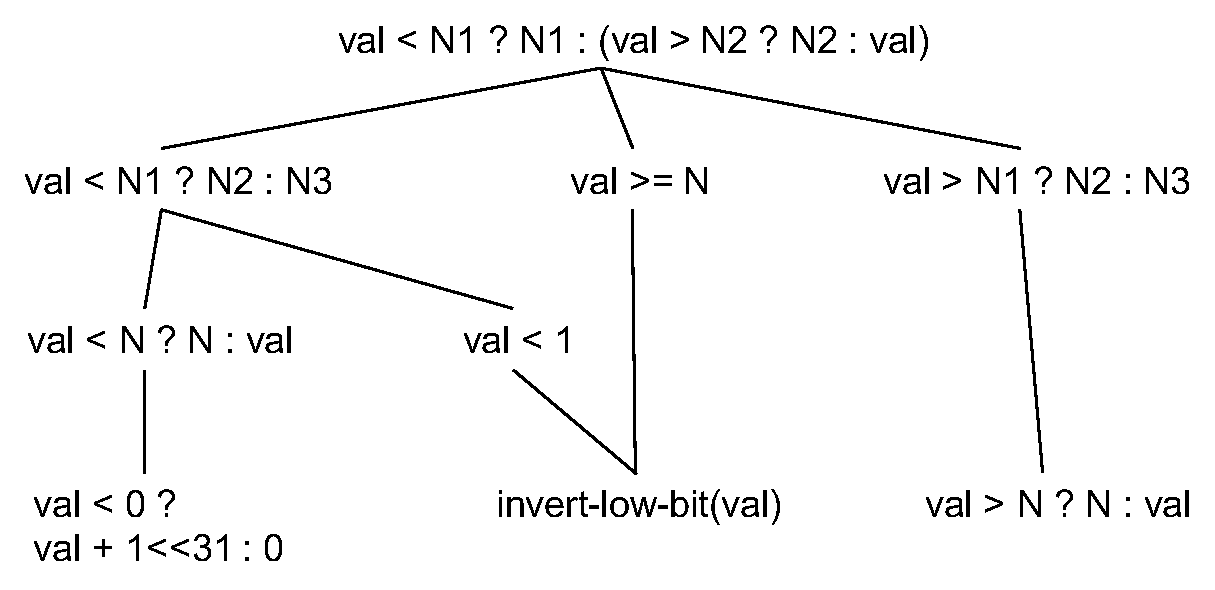
\includegraphics[width=\widthfactor\columnwidth]{chapters/adapter_synthesis/figures/clamp_partial_order}
	\caption{Subset of partial order relationship among adapted clamp instances}
	\label{fig:clamp_partial_order}
\end{figure}
We found that a majority of our generated adapters exploit specific functionality of the reference functions.
%
We explored this observation further by manually summarizing the semantics of the 683 adapters reported for {\tt clamp}.
%
We found that these 683 adapters have a partial order between them created by our adapter families of type conversion and return value substitution.
%
We present a subset of this partial order as a Hasse diagram in
Figure~\ref{fig:clamp_partial_order} with the most general
implementation of {\tt clamp} as the topmost node and functions that use
the most
specific instances of {\tt clamp} at the bottom.
%
To explain one unintuitive example, the {\tt invert-low-bit} operation on a value {\tt v} can be implemented in terms of {\tt val < N} by setting {\tt val} to the low bit of {\tt v} zero-extended to 32 bits and {\tt N} to 1, and zero-extending the low 1 bit of the return value of {\tt val < N} to 32 bits.
%
Some such functionalities owe more to the flexibility of the adapter
family than they do to the reference function.
%
These results suggest it would be worthwhile in the future to prune
them earlier by searching for instances of the simplest reference
functions first, and then excluding these from future searches.

Timeouts were the third possible conclusion of each adapter synthesis task.
The number of timeouts is reported in Table~\ref{table:general}.
%
We show a histogram of the total running time used to find adapters in Figure~\ref{fig:clamp_hist} for the {\tt clamp} reference function.
%
Similar histograms for {\tt tile\_pos} and {\tt median} reference
functions can be found in Section~\ref{sec:histograms}.
%
\subsubsection{Timeouts with {\tt tile\_pos} and {\tt median}}
\label{sec:histograms}
Here we report the histograms of timeouts for the {\tt tile\_pos} and {\tt median} reference functions.
%
Please refer to Figures~\ref{fig:clamp_hist},~\ref{fig:tilepos_hist} and~\ref{fig:median_hist}.
%
\begin{figure}[ht]
    \centering
    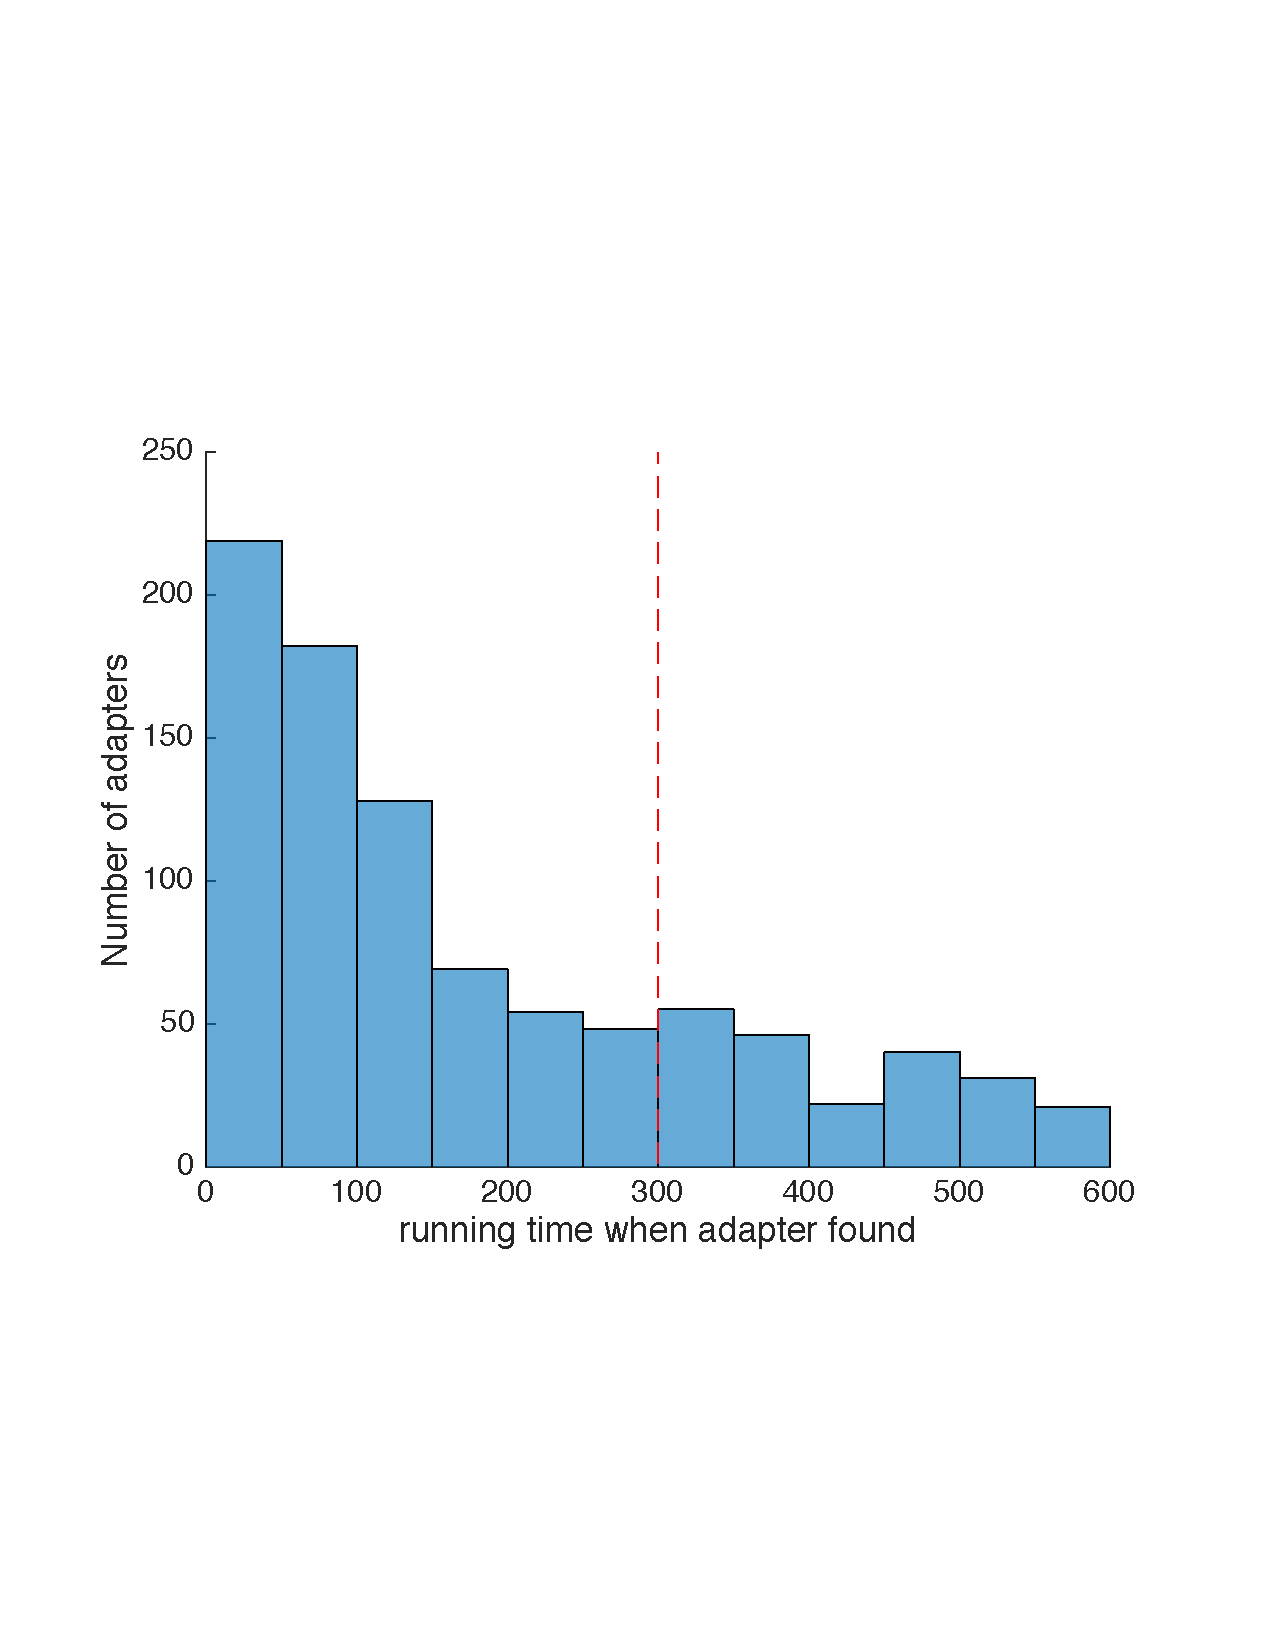
\includegraphics[width=\widthfactor\textwidth]{chapters/adapter_synthesis/figures/clamp_hist}
    \caption{Running times for synthesized adapters using {\tt clamp} reference function}
    \label{fig:clamp_hist}
\end{figure}
\begin{figure}
    \centering
    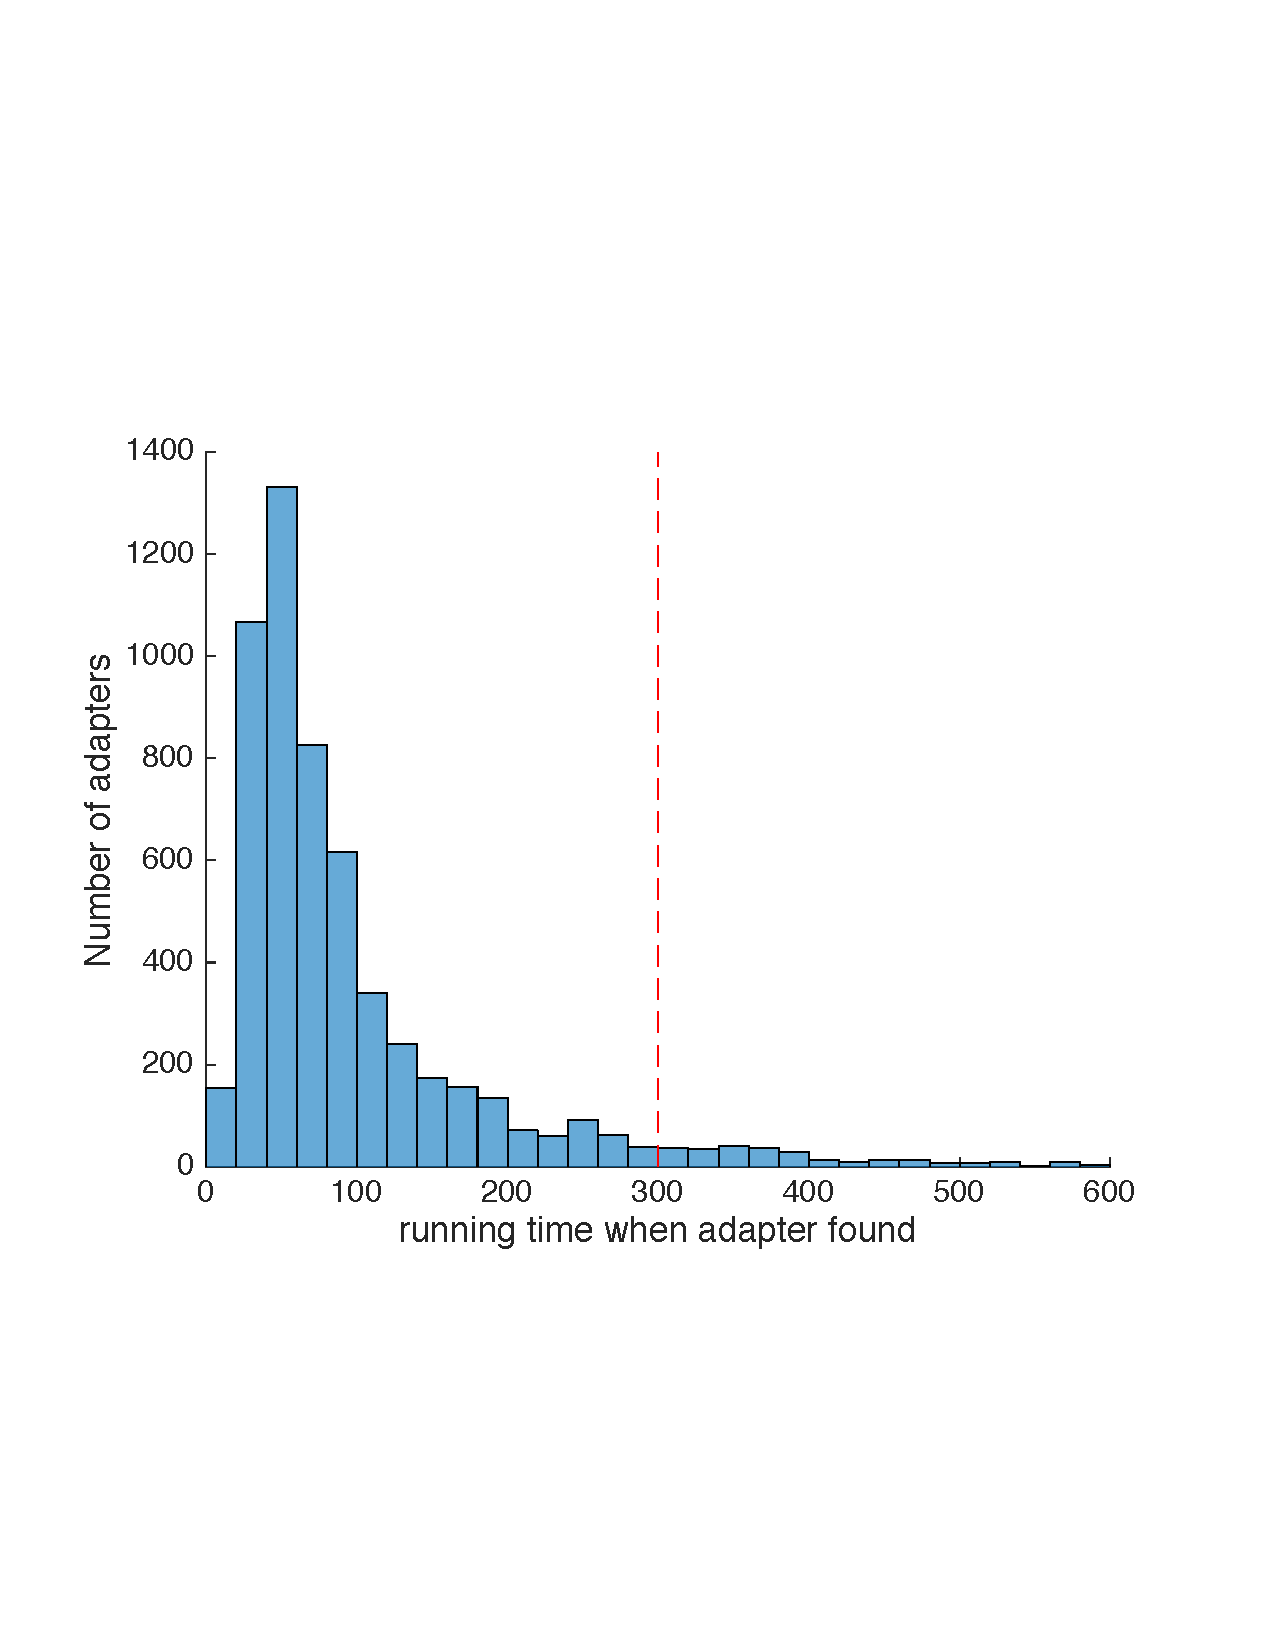
\includegraphics[width=\widthfactor\textwidth]{chapters/adapter_synthesis/figures/tilepos_hist}
    \caption{Running times for synthesized adapters using {\tt tile\_pos} reference function}
    \label{fig:tilepos_hist}
\end{figure}
%
\begin{figure}[ht]
    \centering
    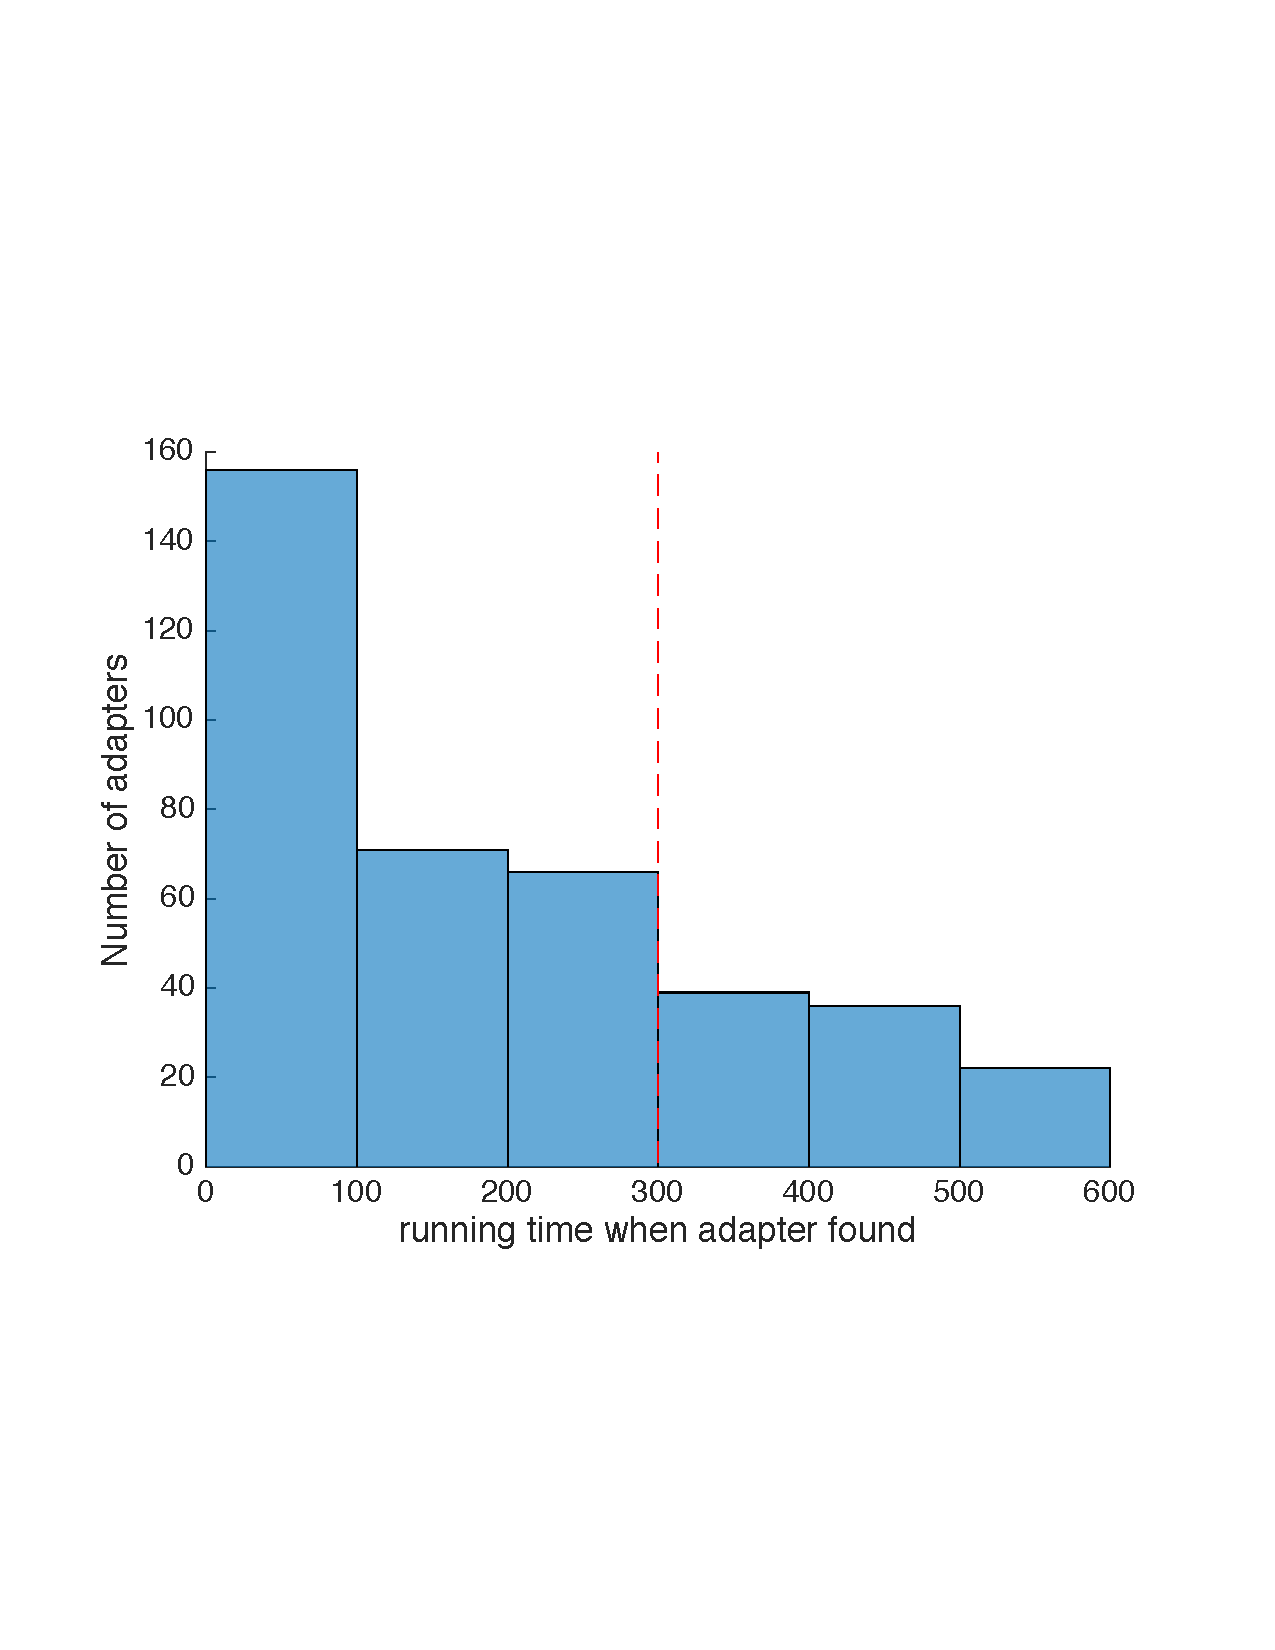
\includegraphics[width=\widthfactor\textwidth]{chapters/adapter_synthesis/figures/median_hist}
    \caption{Running times for synthesized adapters using {\tt median} reference function}
    \label{fig:median_hist}
\end{figure}
%
The number of adapters found after 300 seconds decreases rapidly, consistent with the mean total running time~(subcolumn \textit{total time} under column \textit{adapter} in Table~\ref{table:general}) of 99.3 seconds for the {\tt clamp} reference function.
%
Table~\ref{table:general} also shows that the total running time, when our tool concludes with finding an adapter, is significantly less than 300 seconds for all reference functions that reported adapters.
%
Though setting any finite timeout can cause some instances to be lost,
these results suggest that a 300-second timeout was appropriate for
this experiment, and that most timeouts would not have led to adapters.
%
\subsection{Comparing adapter families}
\label{sec:eval_compare}
%
We also explored the tradeoff between adapter search space size and effectiveness of the adapter family.
%
We ran all 46,831 target code fragments with {\tt clamp} as the reference function using two additional adapter families beyond the combination of type conversion family with return value substitution described above.
%
The first adapter family allowed only argument permutation and the second allowed argument permututation along with substitution with unrestricted 32-bit constants.
%
We ran the first adapter family setup (argument permutation + return value substitution) with a 2.5 minute hard time limit, the second adapter family setup (argument substitution + return value substitution) with a 5 minute hard time limit, and the third adapter family setup (argument substitution + return value substitution) was the same as the previous subsection with also a 5 minute hard time limit.
%
We present our results in Table \ref{table:compare}.
%
\begin{table}
\centering
\caption{Comparing adapter families with 46,831 target code fragments and {\tt clamp} reference function}
\label{table:compare}
\begin{tabular}{|l|l|l|l|l|}
\hline
																 & size           & \#-ad & \#-inequiv & \#-timeout \\ \hline
\begin{tabular}[c]{@{}l@{}}arg\_perm+\\ ret\_sub-2.5m\end{tabular} & 4.98E+10       & 9     & 46803      & 19         \\ \hline
\begin{tabular}[c]{@{}l@{}}arg\_sub+\\ ret\_sub-2.5m\end{tabular}  & 1.3538427E+126 & 705   & 45782      & 344        \\ \hline
\begin{tabular}[c]{@{}l@{}}type\_conv+\\ ret\_sub-5m\end{tabular}  & 1.3538430E+126 & 683   & 40553      & 5595       \\ \hline
\end{tabular}
\end{table}
%
As expected, the number of timeouts increases with an increase in the size of adapter search space.
%
Table \ref{table:compare} also shows that, for {\tt clamp}, a simpler adapter family is better at finding adapters than a more expressive family, because more searches can complete within the timeout.
%
But, this may not be true for all reference functions.
%
Table~\ref{table:compare} suggests that, when computationally feasible, adapter families should be tried in increasing order of expressiveness to have the fewest timeouts overall.
%
We plan to explore this tradeoff between expressiveness and effectiveness of adapter families in the future.

